% Calm Band project report -- compile with XeLaTeX (on Overleaf: Menu > Compiler > XeLaTeX), twice.
\documentclass[12pt,letterpaper,oneside]{report}
\usepackage{fontspec}
\setmainfont{TeX Gyre Termes}          % Times New Roman clone, as in the sample
\setmonofont{DejaVu Sans Mono}[Scale=0.85]
\newfontfamily\rupeefont{DejaVu Sans}
\usepackage{newunicodechar}
\newunicodechar{₹}{{\rupeefont ₹}}
\newunicodechar{→}{\ensuremath{\rightarrow}}
\newunicodechar{↔}{\ensuremath{\leftrightarrow}}
\newunicodechar{≥}{\ensuremath{\geq}}
\newunicodechar{±}{\ensuremath{\pm}}
\usepackage[left=1.18in,right=0.88in,top=0.85in,bottom=0.9in,footskip=0.45in]{geometry}
\usepackage{setspace}
\usepackage{amsmath}
\usepackage{graphicx}
\usepackage[table]{xcolor}
\usepackage{array,tabularx,longtable}
\usepackage{float}
\usepackage{enumitem}
\usepackage{titlesec}
\usepackage{caption}
\usepackage{listings}
\usepackage{fancyhdr}
\usepackage{xurl}
\usepackage[hidelinks]{hyperref}

\definecolor{headgray}{HTML}{DCE6E8}
\definecolor{totalgray}{HTML}{F2F5F5}
\definecolor{codebg}{HTML}{F2F4F5}
\graphicspath{{fig/}}

% Body text: 12 pt, 1.5 line spacing, justified, space between paragraphs (as in the sample).
\onehalfspacing
\setlength{\parindent}{0pt}
\setlength{\parskip}{8pt plus 2pt}
\setlength{\emergencystretch}{3em}
\hyphenpenalty=10000 \exhyphenpenalty=10000 \tolerance=2000   % no hyphenation, as in the sample

% Chapter heading: "CHAPTER n" and title, centred, bold 16 pt.
\titleformat{\chapter}[display]{\centering\bfseries\fontsize{16}{22}\selectfont}{CHAPTER \thechapter}{10pt}{\MakeUppercase}
\titlespacing*{\chapter}{0pt}{24pt}{24pt}
% Section heading: "1.1 Overview", bold 13 pt.
\titleformat{\section}{\bfseries\fontsize{13}{18}\selectfont}{\thesection}{0.5em}{}
\titlespacing*{\section}{0pt}{14pt}{6pt}

% Captions: bold label, 11 pt, centred, "Figure 3.1 Title".
\captionsetup{font={small}, labelfont=bf, labelsep=space, justification=centering, skip=6pt}
\captionsetup[table]{position=top}

\setlist[itemize]{label=\textbullet, leftmargin=*, itemsep=3pt, topsep=4pt}
\setlist[enumerate]{label=\arabic*., leftmargin=*, itemsep=3pt, topsep=4pt}

\lstset{basicstyle=\ttfamily\footnotesize, backgroundcolor=\color{codebg}, breaklines=true, frame=none,
        xleftmargin=6pt, xrightmargin=6pt, aboveskip=6pt, belowskip=6pt, columns=fullflexible, keepspaces=true}

\pagestyle{fancy}\fancyhf{}\renewcommand{\headrulewidth}{0pt}\fancyfoot[C]{\small\thepage}
\fancypagestyle{plain}{\fancyhf{}\renewcommand{\headrulewidth}{0pt}\fancyfoot[C]{\small\thepage}}

\newcommand{\fronttitle}[1]{\begin{center}{\bfseries\fontsize{16}{22}\selectfont #1}\end{center}\vspace{10pt}}
\newcolumntype{Y}{>{\raggedright\arraybackslash}X}
\renewcommand{\arraystretch}{1.25}

\begin{document}

% ------------------------------------------------------------------ title page (as in the sample)
\begin{titlepage}
\begin{center}
\setstretch{1.15}
{\fontsize{20}{28}\selectfont\bfseries CALM BAND: AN IoT COMPANION FOR\\ GUIDED FACIAL-EXERCISE SESSIONS\\ WITH PULSE SENSING AND HAPTIC CUES\par}
\vspace{4pt}
{\fontsize{16}{20}\selectfont\bfseries\itshape 21CSE253T - INTERNET OF THINGS\par}
\vspace{14pt}
A PROJECT REPORT\\[6pt]
\textit{Submitted by}\\[6pt]
{\fontsize{14}{20}\selectfont\bfseries Arnav Bansal\ \ [Reg No: RA2311003010948]}\\[4pt]
{\fontsize{14}{20}\selectfont\bfseries Asmi Sharma\ \ [Reg No: RA2311003010971]}\\[4pt]
{\fontsize{14}{20}\selectfont\bfseries Sarthak Lal\ \ [Reg No: RA2311003010991]}\\[4pt]
\textit{Under the Guidance of}\\[4pt]
{\fontsize{14}{20}\selectfont\bfseries Dr. Arulalan V}\\[2pt]
{\small Department of Computing Technologies}\\[10pt]
\textit{in partial fulfillment of the requirements for the degree of}\\[10pt]
{\fontsize{14}{20}\selectfont\bfseries BACHELOR OF TECHNOLOGY}\\[4pt]
{\fontsize{14}{20}\selectfont\bfseries in}\\[4pt]
{\fontsize{14}{20}\selectfont\bfseries COMPUTER SCIENCE AND ENGINEERING}\\[18pt]

\includegraphics[width=2.44in]{srm_logo.png}\\[18pt]
{\fontsize{14}{22}\selectfont\bfseries DEPARTMENT OF COMPUTING TECHNOLOGIES\\
COLLEGE OF ENGINEERING AND TECHNOLOGY\\
SRM INSTITUTE OF SCIENCE AND TECHNOLOGY\\
KATTANKULATHUR -- 603 203\\[6pt]
November 2026}
\end{center}
\end{titlepage}

\pagenumbering{roman}
\fronttitle{ABSTRACT}\label{abs}
{\fontsize{14}{18.4}\selectfont\setlength{\parskip}{5pt}
Facial-exercise programmes are widely recommended for facial weakness, asymmetry and muscle re-education, but they are usually practised alone at home, where effort, tension and stress go unobserved. \textbf{MirrorWell}, an on-device facial-exercise web application, already counts repetitions and detects over-effort from the camera without sending any video off the device. What it cannot see is the body's response: the pulse, whether the arm is still enough for a clean reading, and whether a gentle, eyes-free cue to ease off is needed.

This project presents the \textbf{Calm Band}, a low-cost Internet of Things (IoT) companion to MirrorWell. An \textbf{ESP32} desk hub reads a \textbf{MAX30102} optical pulse sensor on the fingertip at 100 samples per second and an \textbf{MPU6050} motion sensor on the wrist at 32 samples per second, and drives a \textbf{vibration motor} on the wrist. Every 15 seconds the hub summarises the last 60 seconds into a \textbf{feature window} (finger contact, pulse rate, motion and a quality score) and publishes it over \textbf{MQTT} with TLS to a \textbf{FastAPI} backend. The backend links readings to MirrorWell sessions by their own timestamps, decides whether a reading is fit to show, and turns repetition and ease-off events into short, expiring vibration commands. A physical STOP button cuts the motor instantly, without the network.

Safety and data honesty were first-class requirements: missing data is reported as missing and never as calm, readings that overlap a vibration or a finger removal are withheld, and stale, duplicate, malformed or late commands are rejected on the band itself. The firmware compiles for the ESP32 (69\% of flash, 35\% of RAM) and was validated with \textbf{117 automated checks} across four test suites, all passing, plus two emulator self-tests. A physical prototype then passed every end-to-end test with MirrorWell; a live band card and a reviewer page were added and tested with a simulated band. An encrypted broker and band validation of a WESAD-trained stress model are future work. Hardware cost is ₹949–1,449 (budget ₹1,500).

}
\clearpage
\fronttitle{TABLE OF CONTENTS}\label{toc}
{\setstretch{1.05}
\begin{longtable}{@{}p{0.08\linewidth}p{0.76\linewidth}>{\raggedleft\arraybackslash}p{0.1\linewidth}@{}}
\textbf{} & \textbf{ABSTRACT} & \textbf{\pageref{abs}} \\
\textbf{} & \textbf{LIST OF TABLES} & \textbf{\pageref{lot}} \\
\textbf{} & \textbf{LIST OF FIGURES} & \textbf{\pageref{lof}} \\
\textbf{} & \textbf{LIST OF SYMBOLS AND ABBREVIATIONS} & \textbf{\pageref{abbr}} \\
\textbf{1} & \textbf{INTRODUCTION} & \textbf{\pageref{ch:1}} \\
 & \hspace{1.2em}{\small Overview} & {\small\pageref{sec:1.1}} \\
 & \hspace{1.2em}{\small Motivation} & {\small\pageref{sec:1.2}} \\
 & \hspace{1.2em}{\small Problem Statement} & {\small\pageref{sec:1.3}} \\
 & \hspace{1.2em}{\small Objectives of the Study} & {\small\pageref{sec:1.4}} \\
 & \hspace{1.2em}{\small Scope of the Study} & {\small\pageref{sec:1.5}} \\
 & \hspace{1.2em}{\small Significance of the Study} & {\small\pageref{sec:1.6}} \\
\textbf{2} & \textbf{LITERATURE SURVEY} & \textbf{\pageref{ch:2}} \\
 & \hspace{1.2em}{\small IoT in Healthcare} & {\small\pageref{sec:2.1}} \\
 & \hspace{1.2em}{\small Photoplethysmography and Wearable Pulse Sensing} & {\small\pageref{sec:2.2}} \\
 & \hspace{1.2em}{\small Stress and Heart Rate Variability} & {\small\pageref{sec:2.3}} \\
 & \hspace{1.2em}{\small Motion Artefacts and Signal Quality} & {\small\pageref{sec:2.4}} \\
 & \hspace{1.2em}{\small Haptic Cues and Biofeedback} & {\small\pageref{sec:2.5}} \\
 & \hspace{1.2em}{\small Facial Exercise Therapy and MirrorWell} & {\small\pageref{sec:2.6}} \\
 & \hspace{1.2em}{\small Research Gap} & {\small\pageref{sec:2.7}} \\
\textbf{3} & \textbf{ARCHITECTURE AND DESIGN OF THE CALM BAND SYSTEM} & \textbf{\pageref{ch:3}} \\
 & \hspace{1.2em}{\small System Architecture and Components} & {\small\pageref{sec:3.1}} \\
 & \hspace{1.2em}{\small Workflow of the System} & {\small\pageref{sec:3.2}} \\
 & \hspace{1.2em}{\small Technology Stack} & {\small\pageref{sec:3.3}} \\
 & \hspace{1.2em}{\small Hardware Design and Physical Layout} & {\small\pageref{sec:3.4}} \\
 & \hspace{1.2em}{\small Firmware Design} & {\small\pageref{sec:3.5}} \\
 & \hspace{1.2em}{\small Backend and Companion Design} & {\small\pageref{sec:3.6}} \\
\textbf{4} & \textbf{METHODOLOGY FOR SENSING, SIGNAL QUALITY AND HAPTIC CUES} & \textbf{\pageref{ch:4}} \\
 & \hspace{1.2em}{\small Sampling and Feature Windows} & {\small\pageref{sec:4.1}} \\
 & \hspace{1.2em}{\small Contact, Pulse and Motion Features} & {\small\pageref{sec:4.2}} \\
 & \hspace{1.2em}{\small Signal Quality and Eligibility Rules} & {\small\pageref{sec:4.3}} \\
 & \hspace{1.2em}{\small Command Protocol and Safety Checks} & {\small\pageref{sec:4.4}} \\
 & \hspace{1.2em}{\small Programming Languages and Libraries Used} & {\small\pageref{sec:4.5}} \\
 & \hspace{1.2em}{\small Planned Stress Estimation (Machine Learning)} & {\small\pageref{sec:4.6}} \\
\textbf{5} & \textbf{IMPLEMENTATION OF THE PROJECT} & \textbf{\pageref{ch:5}} \\
 & \hspace{1.2em}{\small Firmware Implementation} & {\small\pageref{sec:5.1}} \\
 & \hspace{1.2em}{\small MQTT Interface} & {\small\pageref{sec:5.2}} \\
 & \hspace{1.2em}{\small Backend Implementation} & {\small\pageref{sec:5.3}} \\
 & \hspace{1.2em}{\small MirrorWell Companion Bridge} & {\small\pageref{sec:5.4}} \\
 & \hspace{1.2em}{\small Simulation and Test Harness} & {\small\pageref{sec:5.5}} \\
 & \hspace{1.2em}{\small Iterative Review and Hardening} & {\small\pageref{sec:5.6}} \\
\textbf{6} & \textbf{RESULTS AND DISCUSSION} & \textbf{\pageref{ch:6}} \\
 & \hspace{1.2em}{\small Test Results} & {\small\pageref{sec:6.1}} \\
 & \hspace{1.2em}{\small Resource Usage on the ESP32} & {\small\pageref{sec:6.2}} \\
 & \hspace{1.2em}{\small Emulated-Hardware Results} & {\small\pageref{sec:6.3}} \\
 & \hspace{1.2em}{\small Real Hardware Results} & {\small\pageref{sec:6.hw}} \\
 & \hspace{1.2em}{\small Data Storage in the Backend} & {\small\pageref{sec:6.store}} \\
 & \hspace{1.2em}{\small Live Band Card in MirrorWell} & {\small\pageref{sec:6.live}} \\
 & \hspace{1.2em}{\small Post-Session Summary in Plain Words} & {\small\pageref{sec:6.summary}} \\
 & \hspace{1.2em}{\small Reviewer and Therapist Page} & {\small\pageref{sec:6.reviewer}} \\
 & \hspace{1.2em}{\small Experimental Calm Index} & {\small\pageref{sec:6.calm}} \\
 & \hspace{1.2em}{\small Experimental Stress Model (WESAD)} & {\small\pageref{sec:6.stress}} \\
 & \hspace{1.2em}{\small Testing of the New Parts} & {\small\pageref{sec:6.newtests}} \\
 & \hspace{1.2em}{\small Discussion} & {\small\pageref{sec:6.4}} \\
 & \hspace{1.2em}{\small Limitations} & {\small\pageref{sec:6.5}} \\
\textbf{7} & \textbf{CONCLUSION AND FUTURE SCOPE} & \textbf{\pageref{ch:7}} \\
 & \hspace{1.2em}{\small Conclusion} & {\small\pageref{sec:7.1}} \\
 & \hspace{1.2em}{\small Future Scope} & {\small\pageref{sec:7.2}} \\
\textbf{} & \textbf{REFERENCES} & \textbf{\pageref{refs}} \\
\textbf{} & \textbf{APPENDICES} & \textbf{\pageref{appx}} \\
 & \hspace{1.2em}{\small Appendix 1: Message Formats} & {\small\pageref{sec:appendix-1-message-formats}} \\
 & \hspace{1.2em}{\small Appendix 2: Bill of Materials} & {\small\pageref{sec:appendix-2-bill-of-materials}} \\
 & \hspace{1.2em}{\small Paper Publication Proof} & {\small\pageref{sec:paper-publication-proof}} \\
 & \hspace{1.2em}{\small Plagiarism Report} & {\small\pageref{sec:plagiarism-report}} \\
\end{longtable}}
\clearpage
\fronttitle{LIST OF TABLES}\label{lot}
{\small\setstretch{1.3}
\noindent\makebox[0.09\linewidth][l]{\ref{tab:hardware-components-and-their-roles}}Hardware Components and Their Roles\dotfill\pageref{tab:hardware-components-and-their-roles}\par
\noindent\makebox[0.09\linewidth][l]{\ref{tab:technology-stack}}Technology Stack\dotfill\pageref{tab:technology-stack}\par
\noindent\makebox[0.09\linewidth][l]{\ref{tab:pin-assignment-on-the-esp32}}Pin Assignment on the ESP32\dotfill\pageref{tab:pin-assignment-on-the-esp32}\par
\noindent\makebox[0.09\linewidth][l]{\ref{tab:sampling-and-window-parameters}}Sampling and Window Parameters\dotfill\pageref{tab:sampling-and-window-parameters}\par
\noindent\makebox[0.09\linewidth][l]{\ref{tab:status-rules-applied-by-the-backend-in-o}}Status Rules Applied by the Backend (in order)\dotfill\pageref{tab:status-rules-applied-by-the-backend-in-o}\par
\noindent\makebox[0.09\linewidth][l]{\ref{tab:vibration-patterns}}Vibration Patterns\dotfill\pageref{tab:vibration-patterns}\par
\noindent\makebox[0.09\linewidth][l]{\ref{tab:mqtt-topics}}MQTT Topics\dotfill\pageref{tab:mqtt-topics}\par
\noindent\makebox[0.09\linewidth][l]{\ref{tab:backend-http-endpoints}}Backend HTTP Endpoints\dotfill\pageref{tab:backend-http-endpoints}\par
\noindent\makebox[0.09\linewidth][l]{\ref{tab:main-findings-from-the-review-rounds}}Main Findings from the Review Rounds\dotfill\pageref{tab:main-findings-from-the-review-rounds}\par
\noindent\makebox[0.09\linewidth][l]{\ref{tab:automated-test-results}}Automated Test Results\dotfill\pageref{tab:automated-test-results}\par
\noindent\makebox[0.09\linewidth][l]{\ref{tab:firmware-size}}Firmware Size\dotfill\pageref{tab:firmware-size}\par
\noindent\makebox[0.09\linewidth][l]{\ref{tab:hardware-bring-up-checks}}Hardware Bring-up Checks\dotfill\pageref{tab:hardware-bring-up-checks}\par
\noindent\makebox[0.09\linewidth][l]{\ref{tab:bench-mode-pulse-readings}}BENCH-Mode Pulse Readings with a Still Fingertip\dotfill\pageref{tab:bench-mode-pulse-readings}\par
\noindent\makebox[0.09\linewidth][l]{\ref{tab:end-to-end-results-real-hardware}}End-to-End Results on the Real Hardware\dotfill\pageref{tab:end-to-end-results-real-hardware}\par
\noindent\makebox[0.09\linewidth][l]{\ref{tab:live-card-messages}}Messages Shown on the Live Card\dotfill\pageref{tab:live-card-messages}\par
\noindent\makebox[0.09\linewidth][l]{\ref{tab:stress-model-results}}Leave-One-Subject-Out Results of the Experimental Stress Model on WESAD\dotfill\pageref{tab:stress-model-results}\par
\noindent\makebox[0.09\linewidth][l]{\ref{tab:new-tests}}Automated Tests of the Storage, Live Card, Summary and Reviewer Parts\dotfill\pageref{tab:new-tests}\par
\noindent\makebox[0.09\linewidth][l]{\ref{tab:bill-of-materials-estimated-prices-octob}}Bill of Materials (estimated prices, October 2026)\dotfill\pageref{tab:bill-of-materials-estimated-prices-octob}\par
}
\clearpage
\fronttitle{LIST OF FIGURES}\label{lof}
{\small\setstretch{1.3}
\noindent\makebox[0.09\linewidth][l]{\ref{fig:diag_arch}}Architecture Diagram of the System\dotfill\pageref{fig:diag_arch}\par
\noindent\makebox[0.09\linewidth][l]{\ref{fig:diag_seq}}Session Workflow for One Repetition\dotfill\pageref{fig:diag_seq}\par
\noindent\makebox[0.09\linewidth][l]{\ref{fig:render_hero}}3D Render of the Calm Band (Desk Hub, Wrist Strap and Fingertip Sensor)\dotfill\pageref{fig:render_hero}\par
\noindent\makebox[0.09\linewidth][l]{\ref{fig:render_closeups}}Close-up Renders of the Three Units\dotfill\pageref{fig:render_closeups}\par
\noindent\makebox[0.09\linewidth][l]{\ref{fig:wiring}}Wiring Diagram of the Calm Band\dotfill\pageref{fig:wiring}\par
\noindent\makebox[0.09\linewidth][l]{\ref{fig:chart_windows}}Overlapping Feature Windows and Their Eligibility\dotfill\pageref{fig:chart_windows}\par
\noindent\makebox[0.09\linewidth][l]{\ref{fig:diag_gate}}Command Checks on the Band\dotfill\pageref{fig:diag_gate}\par
\noindent\makebox[0.09\linewidth][l]{\ref{fig:chart_tests}}Growth of the Automated Test Suites\dotfill\pageref{fig:chart_tests}\par
\noindent\makebox[0.09\linewidth][l]{\ref{fig:chart_selftest}}Motor Self-Test on the Emulated ESP32\dotfill\pageref{fig:chart_selftest}\par
\noindent\makebox[0.09\linewidth][l]{\ref{fig:ui_live_cue}}Live Band Card Showing the Heart, Signal Bars and Steadiness During a Cue\dotfill\pageref{fig:ui_live_cue}\par
\noindent\makebox[0.09\linewidth][l]{\ref{fig:ui_live_moving}}Live Card When the Hand Is Moving\dotfill\pageref{fig:ui_live_moving}\par
\noindent\makebox[0.09\linewidth][l]{\ref{fig:ui_live_contact}}Live Card When the Finger Is Off the Sensor\dotfill\pageref{fig:ui_live_contact}\par
\noindent\makebox[0.09\linewidth][l]{\ref{fig:ui_summary}}Post-Session Summary in Plain Words\dotfill\pageref{fig:ui_summary}\par
\noindent\makebox[0.09\linewidth][l]{\ref{fig:rev_list}}Reviewer Page: Session List, Session Facts and Trends\dotfill\pageref{fig:rev_list}\par
\noindent\makebox[0.09\linewidth][l]{\ref{fig:rev_timeline}}Reviewer Page: Session Timeline with Gaps, Buzz and Movement Shading and Markers\dotfill\pageref{fig:rev_timeline}\par
}
\clearpage
\fronttitle{LIST OF SYMBOLS AND ABBREVIATIONS}\label{abbr}
\begin{tabular}{@{}p{0.18\linewidth}p{0.78\linewidth}@{}}
\textbf{ACK} & Acknowledgement message from the band \\
\textbf{API} & Application Programming Interface \\
\textbf{BLE} & Bluetooth Low Energy \\
\textbf{BPM} & Beats Per Minute \\
\textbf{FIFO} & First-In, First-Out buffer \\
\textbf{GPIO} & General-Purpose Input/Output pin \\
\textbf{HRV} & Heart Rate Variability \\
\textbf{HTTP(S)} & Hypertext Transfer Protocol (Secure) \\
\textbf{I²C} & Inter-Integrated Circuit, a two-wire sensor bus \\
\textbf{IBI} & Inter-Beat Interval, the time between two heartbeats \\
\textbf{IoT} & Internet of Things \\
\textbf{IR} & Infrared \\
\textbf{JSON} & JavaScript Object Notation \\
\textbf{ML} & Machine Learning \\
\textbf{MQTT} & Message Queuing Telemetry Transport, a light publish/subscribe protocol \\
\textbf{NTP} & Network Time Protocol \\
\textbf{PPG} & Photoplethysmography, optical measurement of blood-volume pulse \\
\textbf{PWA} & Progressive Web Application \\
\textbf{QEMU} & Quick Emulator, used here to emulate the ESP32 \\
\textbf{QoS} & Quality of Service level in MQTT \\
\textbf{RAM} & Random-Access Memory \\
\textbf{RMS} & Root Mean Square \\
\textbf{TLS} & Transport Layer Security \\
\textbf{TTL} & Time To Live, how long a command stays valid \\
\textbf{WESAD} & Wearable Stress and Affect Detection dataset \\
\end{tabular}
\clearpage
\pagenumbering{arabic}

\chapter{INTRODUCTION}\label{ch:1}

\section{Overview}\label{sec:1.1}

The Internet of Things connects small sensing devices to software that can store, analyse and act on what they measure. In healthcare, this makes it possible to observe a person's body continuously and cheaply outside a clinic, using low-power microcontrollers, standard wireless networks and cloud services [1], [2]. Wearable optical pulse sensors, based on \textbf{photoplethysmography (PPG)}, are now found in almost every fitness band and are well understood as a way to measure heart rate from the skin [3], [4].


\textbf{MirrorWell} is an existing facial-exercise application developed by the team. It runs entirely in the browser: the camera image is processed on the device with MediaPipe face tracking [5], repetitions and over-effort are counted from facial landmarks, and no video or landmark data ever leaves the device. The application already knows when a session starts, when each repetition happens and when the user should ease off. It does not know how the user's body is responding.


This project, the \textbf{Calm Band}, adds that missing view. It is a small IoT system made of a desk hub (an ESP32 microcontroller on two mini breadboards), a wrist strap carrying a motion sensor and a vibration motor, and a fingertip sensor that measures pulse. The hub publishes compact summaries of the user's pulse, motion and signal quality to a backend, and the backend sends back short vibration cues that follow the exercise. MirrorWell gains an opt-in \textbf{companion mode} that shows the live status and stores a summary of each session for later review.


\section{Motivation}\label{sec:1.2}

Facial-exercise therapy is commonly prescribed for facial palsy and similar conditions, and controlled studies report benefit when exercises are performed regularly and correctly [6]. Most practice, however, happens at home without a therapist. Two problems follow. First, users tend to over-strain, and strain shows up in the body (a rising pulse, tension) before it is obvious on the face. Second, the user's eyes are on the screen and their own face, so audio prompts or pop-ups interrupt the exercise, while a short vibration on the wrist does not.


Stress itself is measurable: heart rate and heart rate variability change in a consistent way under mental stress [7], and public datasets such as WESAD make it possible to train stress classifiers on wrist-worn signals [8]. A low-cost band that collects clean pulse data during and around exercise sessions is therefore useful both now (for live feedback and review) and later (as input to a stress-estimation model).


Finally, the project had firm practical constraints: a hardware budget of about ₹1,000–1,500, parts available in India within days, a breadboard-level build that a student team can assemble, and no change to MirrorWell's rule that camera data stays on the device.


\section{Problem Statement}\label{sec:1.3}

Home facial-exercise practice lacks an objective, low-cost signal of how the user's body is responding, and lacks a non-visual way to guide the user during the exercise. A solution must measure pulse and motion reliably enough to be trusted, deliver timely haptic cues that can never fire late or run on, link the measurements to MirrorWell sessions without weakening MirrorWell's privacy guarantees, and do all of this with commodity parts within a student budget. Above all, it must \textbf{never present missing or corrupted data as a calm, normal reading}.


\section{Objectives of the Study}\label{sec:1.4}

The main objective is to design, build and validate an IoT companion that measures pulse and motion during MirrorWell sessions and provides safe haptic cues. The specific objectives are:


\begin{enumerate}\item \textbf{Sensing:} read fingertip pulse at 100 Hz and wrist motion at 32 Hz on an ESP32, and summarise them every 15 seconds into 60-second feature windows with explicit contact, motion and quality flags.
\item \textbf{Reliable delivery:} publish readings over MQTT with TLS, queue up to 30 minutes of readings while offline, and resend them with their original timestamps.
\item \textbf{Safe haptic cues:} map repetition and ease-off events to short vibration patterns (at most 1.5 seconds) that are rejected if malformed, duplicated or expired, plus a STOP button that works without the network.
\item \textbf{Honest status:} show a pulse value only when the reading is recent, from the current device boot, with good contact, no motion, no vibration overlap and no timing gaps.
\item \textbf{Integration:} add an opt-in companion mode to MirrorWell that sends only numeric session events, never camera data.
\item \textbf{Verification:} build automated tests, a simulated band and emulator self-tests so the system can be validated before and alongside the physical build.
\end{enumerate}

\section{Scope of the Study}\label{sec:1.5}

\begin{itemize}\item \textbf{Hardware:} one ESP32 DevKit V1 (30-pin), one MAX30102 pulse sensor, one MPU6050 motion sensor, one vibration motor module and one STOP button, assembled on breadboards in a desk-hub layout.
\item \textbf{Firmware:} sampling, feature windows, signal-quality rules, command validation, vibration patterns, offline queue and sensor health reporting on the ESP32.
\item \textbf{Backend:} a FastAPI service that receives readings over MQTT, validates every message, applies status rules, manages sessions and issues vibration commands.
\item \textbf{Application:} the MirrorWell companion bridge, limited to session events and summaries.
\item \textbf{Out of scope for this phase:} medical diagnosis, all-day wear, and the stress-estimation model, which is planned as Phase 2 using the WESAD dataset.
\end{itemize}

\section{Significance of the Study}\label{sec:1.6}

\begin{itemize}\item It shows how a \textbf{sub-₹1,500} IoT design can add physiological feedback to an existing, privacy-first health application without moving camera data off the device.
\item It treats \textbf{data quality as part of the design}: every reading carries flags that explain why it can or cannot be trusted.
\item It demonstrates \textbf{safety-aware actuation}: vibration commands expire, cannot repeat, cannot run longer than 1.5 seconds, and can always be stopped locally.
\item It provides a \textbf{tested, documented baseline} (117 automated checks) on which hardware validation and the planned stress model can build.
\end{itemize}

The following chapters review related work, describe the architecture and design, explain the methods used for sensing and cueing, detail the implementation, and present the results obtained so far.


\chapter{LITERATURE SURVEY}\label{ch:2}

\section{IoT in Healthcare}\label{sec:2.1}

Atzori et al. describe the IoT as the combination of identifiable sensing devices, network connectivity and middleware that turns raw readings into services [1]. Islam et al. survey IoT healthcare systems and identify three recurring layers: body-worn or bedside sensors, a gateway or hub, and a cloud or server layer that stores, analyses and alerts [2]. They also highlight security, data integrity and reliability as the main open problems. The Calm Band follows this three-layer pattern: the wearable sensors, the ESP32 desk hub as the gateway, and the FastAPI backend with its database. MQTT, standardised by OASIS, is the most common messaging protocol for such systems because it is light, supports publish/subscribe and offers delivery guarantees through Quality of Service levels [9].


\section{Photoplethysmography and Wearable Pulse Sensing}\label{sec:2.2}

Allen reviews PPG as a simple optical technique in which an LED lights the skin and a photodiode measures how much light is absorbed as blood volume changes with each heartbeat [3]. The fingertip gives a strong signal because of its dense blood supply. Elgendi analyses the fingertip PPG waveform and shows that heart rate can be found reliably from the systolic peaks once the slow baseline is removed [10]. Tamura et al. review wearable PPG sensors and note that reflective sensors such as the MAX30102 are now cheap and power-efficient, but remain sensitive to contact pressure and movement [4]. The MAX30102 integrates red and infrared LEDs, a photodetector and an on-chip 32-sample FIFO buffer, and is read over I²C [11].


\section{Stress and Heart Rate Variability}\label{sec:2.3}

Kim et al. performed a meta-analysis of studies on stress and heart rate variability (HRV) and found that stress consistently lowers parasympathetic activity, which appears as reduced beat-to-beat variability [7]. Schmidt et al. released WESAD, a dataset recorded from chest- and wrist-worn devices during baseline, amusement and stress conditions, and showed that classical machine-learning models on such signals can separate stress from non-stress states with useful accuracy [8]. Can et al. survey stress detection in daily life with phones and wearables and conclude that motion artefacts and missing data are the main reasons laboratory accuracy is not reached in practice [12]. These findings shaped two decisions in this project: keep the beat-level timing needed for HRV, and attach explicit quality flags to every reading.


\section{Motion Artefacts and Signal Quality}\label{sec:2.4}

Movement changes how the sensor sits on the skin and adds large, slow changes to the PPG signal that can be mistaken for heartbeats [4], [12]. The common remedies are to measure movement with an accelerometer, to reject or down-weight windows with significant motion, and to check that each beat-to-beat interval falls in a physiologically possible range. The MPU6050 combines a three-axis accelerometer and gyroscope and is widely used for exactly this purpose [13]. The Calm Band applies all three remedies, and adds a fourth that is rarely discussed: a missing motion sensor must not be treated as perfect stillness.


\section{Haptic Cues and Biofeedback}\label{sec:2.5}

Biofeedback presents a person's own physiological signals back to them so they can learn to regulate them [14]. Vibration is attractive in this setting because it does not compete with the visual task. However, an actuator worn on the body must be predictable: a cue that arrives late, repeats, or keeps running is worse than no cue. This motivates the strict command rules in this project (expiry, duplicate rejection, a hard 1.5-second limit and a local STOP button).


\section{Facial Exercise Therapy and MirrorWell}\label{sec:2.6}

Pereira et al. reviewed facial exercise therapy for facial palsy and found evidence that structured exercise improves facial function, especially when practised consistently [6]. MirrorWell supports this practice on a laptop or phone by tracking the face with MediaPipe, which runs in the browser and returns facial landmarks and blendshapes [5]. Because MirrorWell's design forbids any network call from the core application, the companion integration in this project is opt-in, sends only numbers to a same-origin endpoint, and never sends images or landmarks.


\section{Research Gap}\label{sec:2.7}

Commercial fitness bands measure heart rate well, but their data is usually locked inside the vendor's app and cannot drive cues tied to an exercise session. Research systems for stress detection focus on classification accuracy and seldom address how a live system should behave when data is missing, late or disturbed by its own actuator. No low-cost, open system was found that combines pulse and motion sensing, session-linked haptic cues and explicit data-quality rules for home facial-exercise practice. The Calm Band is designed to fill this gap.


\chapter{ARCHITECTURE AND DESIGN OF THE CALM BAND SYSTEM}\label{ch:3}

\section{System Architecture and Components}\label{sec:3.1}

The system has four layers, shown in Figure 3.1. The \textbf{wearable layer} contains the fingertip pulse sensor, the wrist motion sensor, the wrist vibration motor and the STOP button. The \textbf{desk hub} is an ESP32 microcontroller that samples the sensors, builds feature windows, checks commands and drives the motor. The \textbf{network layer} is an MQTT broker (EMQX Cloud, over TLS on port 8883). The \textbf{application layer} is a FastAPI backend with a database (SQLite in the demonstration build; PostgreSQL on Supabase is the planned cloud option), the MirrorWell web application and a reviewer page.


\begin{figure}[H]\centering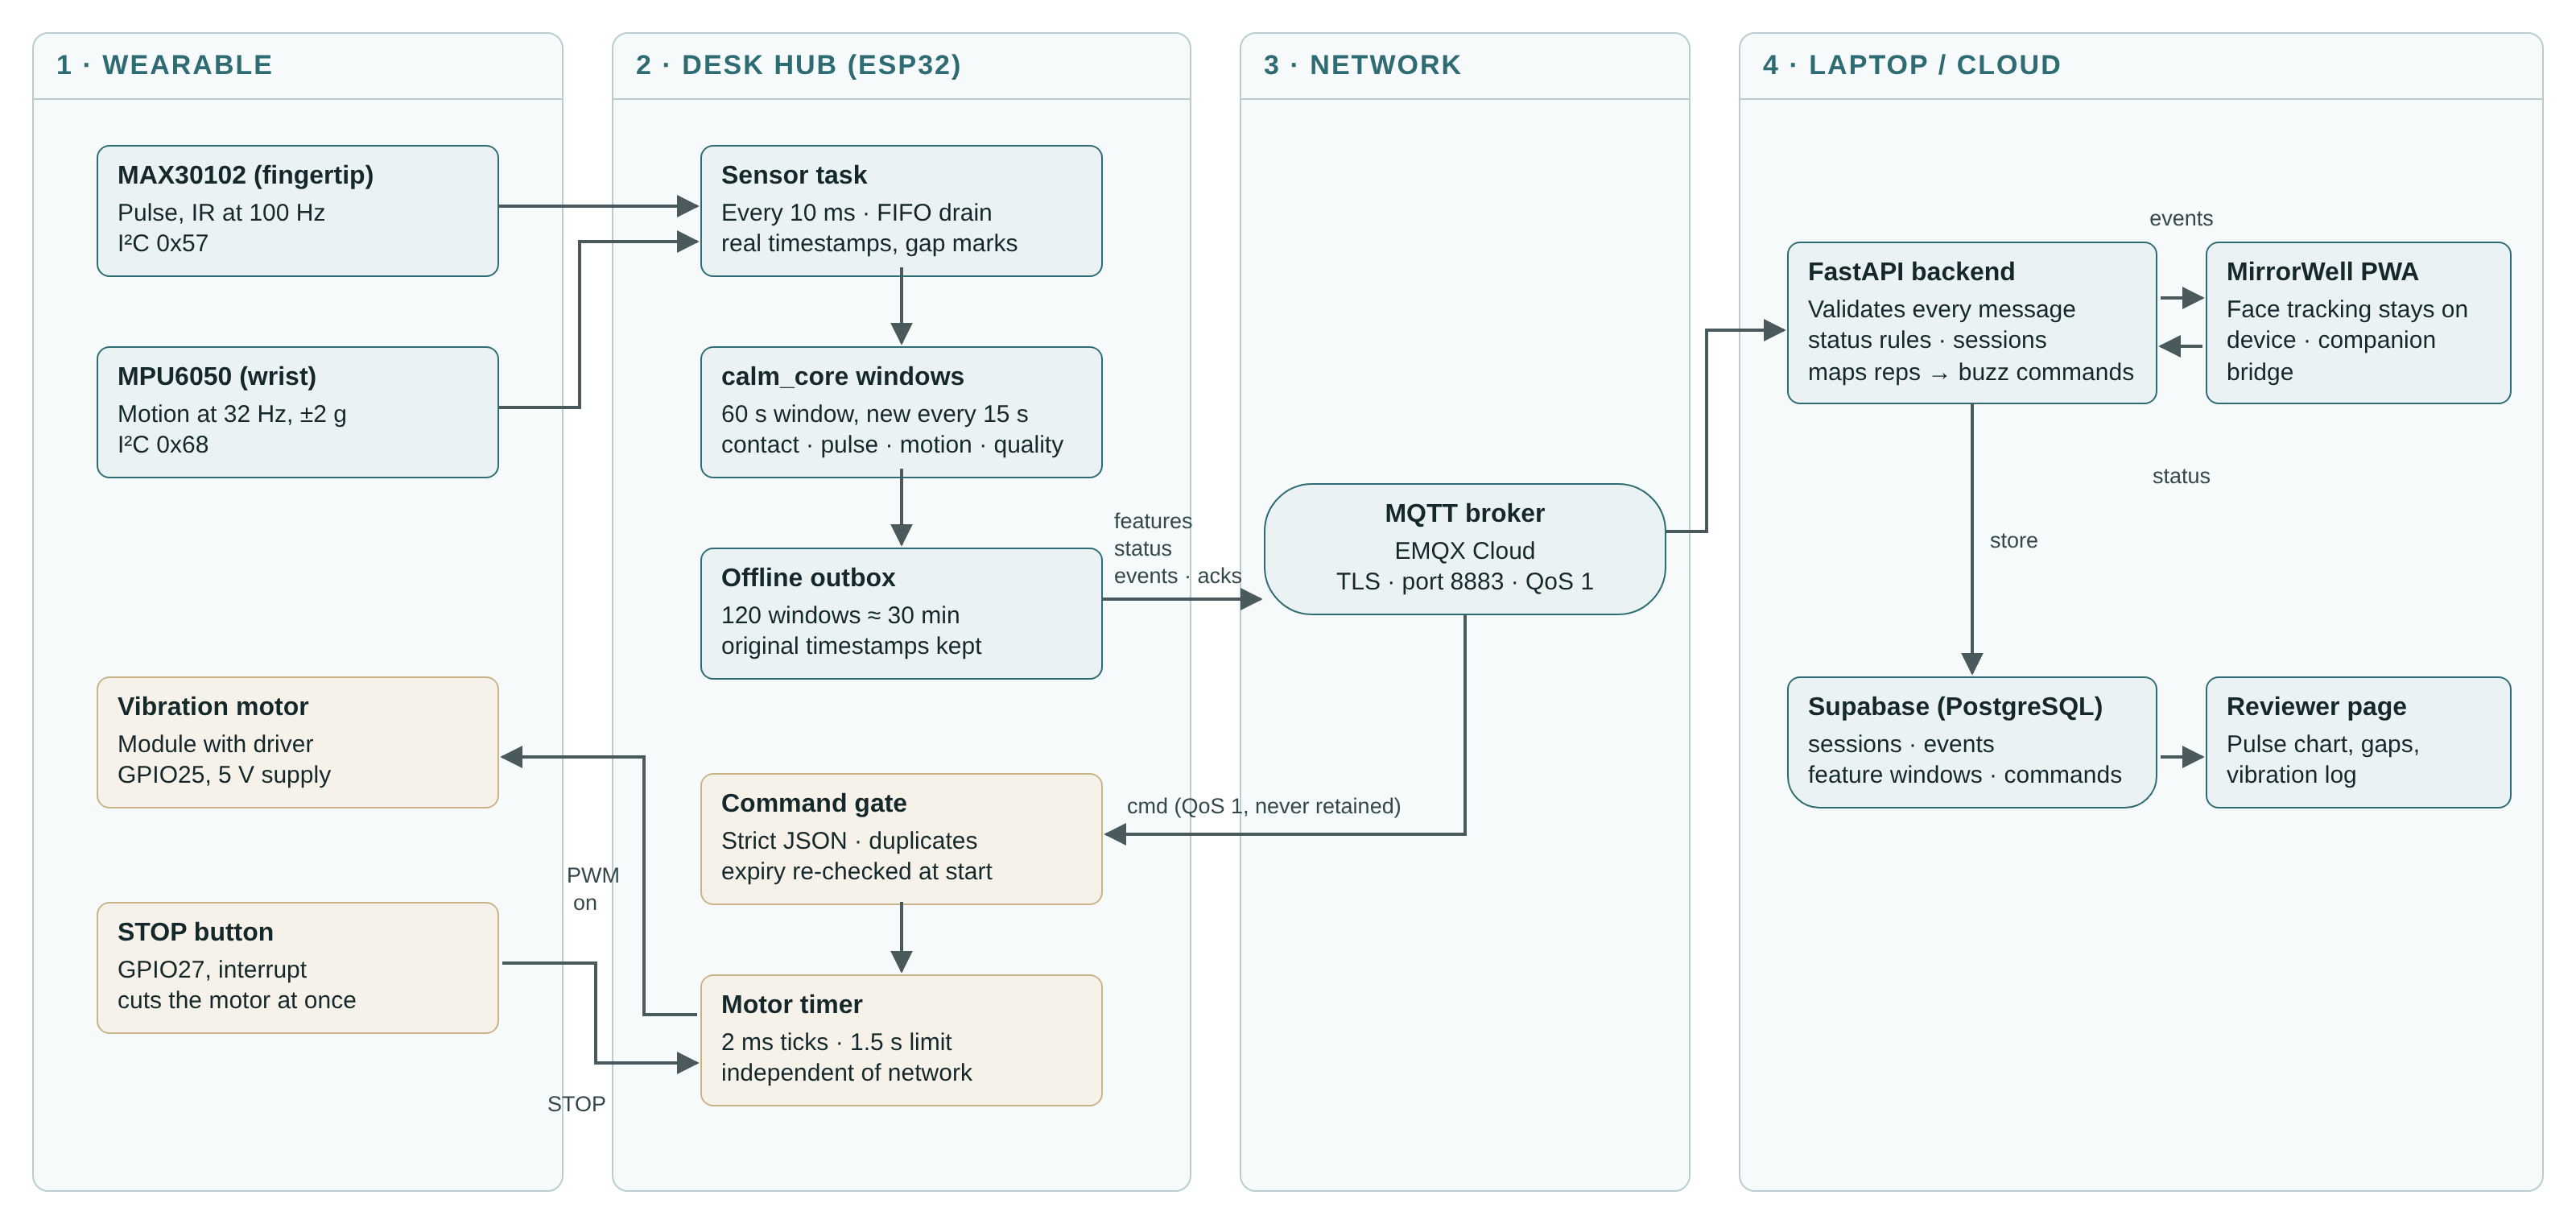
\includegraphics[width=6.3in,height=7.4in,keepaspectratio]{diag_arch.png}\caption{Architecture Diagram of the System}\label{fig:diag_arch}\end{figure}

The components and their roles are listed in Table 3.1. The ESP32 was chosen because it combines Wi-Fi, two processor cores and enough memory for TLS in a ₹400–550 board [15]. The MAX30102 and MPU6050 share one I²C bus at different addresses (0x57 and 0x68), so only two signal wires are needed for both sensors.


\begin{table}[H]
\centering\small\setstretch{1.0}
\caption{Hardware Components and Their Roles}\label{tab:hardware-components-and-their-roles}
\begin{tabular}{|>{\raggedright\arraybackslash}p{\dimexpr 0.330\linewidth-2\tabcolsep-0.4pt\relax}|>{\raggedright\arraybackslash}p{\dimexpr 0.194\linewidth-2\tabcolsep-0.4pt\relax}|>{\raggedright\arraybackslash}p{\dimexpr 0.446\linewidth-2\tabcolsep-0.4pt\relax}|}
\hline
\rowcolor{headgray}\textbf{Component} & \textbf{Interface} & \textbf{Role in the system} \\ \hline
ESP32 DevKit V1 (ESP32-WROOM-32, 30-pin) & USB power, Wi-Fi & Desk hub: sampling, feature windows, MQTT, command checks, motor control \\ \hline
MAX30102 pulse sensor & I²C 0x57, 3.3 V & Fingertip PPG: red and infrared light at 100 samples per second \\ \hline
MPU6050 (GY-521) motion sensor & I²C 0x68, 3.3 V & Wrist movement at 32 samples per second, ±2 g range \\ \hline
Vibration motor module (driver + diode on board) & GPIO25, 5 V supply & Short haptic cues on the wrist \\ \hline
Tactile push button & GPIO27 to GND & STOP: cuts the motor instantly, without the network \\ \hline
On-board LED & GPIO2 & Solid when connected, blinking when not \\ \hline
\end{tabular}
\end{table}

\section{Workflow of the System}\label{sec:3.2}

Figure 3.2 shows what happens during one repetition. MirrorWell detects the repetition and sends a numeric event to the backend. The backend validates it, maps it to a \texttt{rep\_\allowbreak{}pulse} vibration pattern and publishes a command that expires 3 seconds after it was issued. The band validates the command, re-checks the expiry, starts the motor and acknowledges it twice: once when it starts and once when it finishes. Independently, every 15 seconds the band publishes a 60-second feature window, and MirrorWell polls the backend for the current status.


\begin{figure}[H]\centering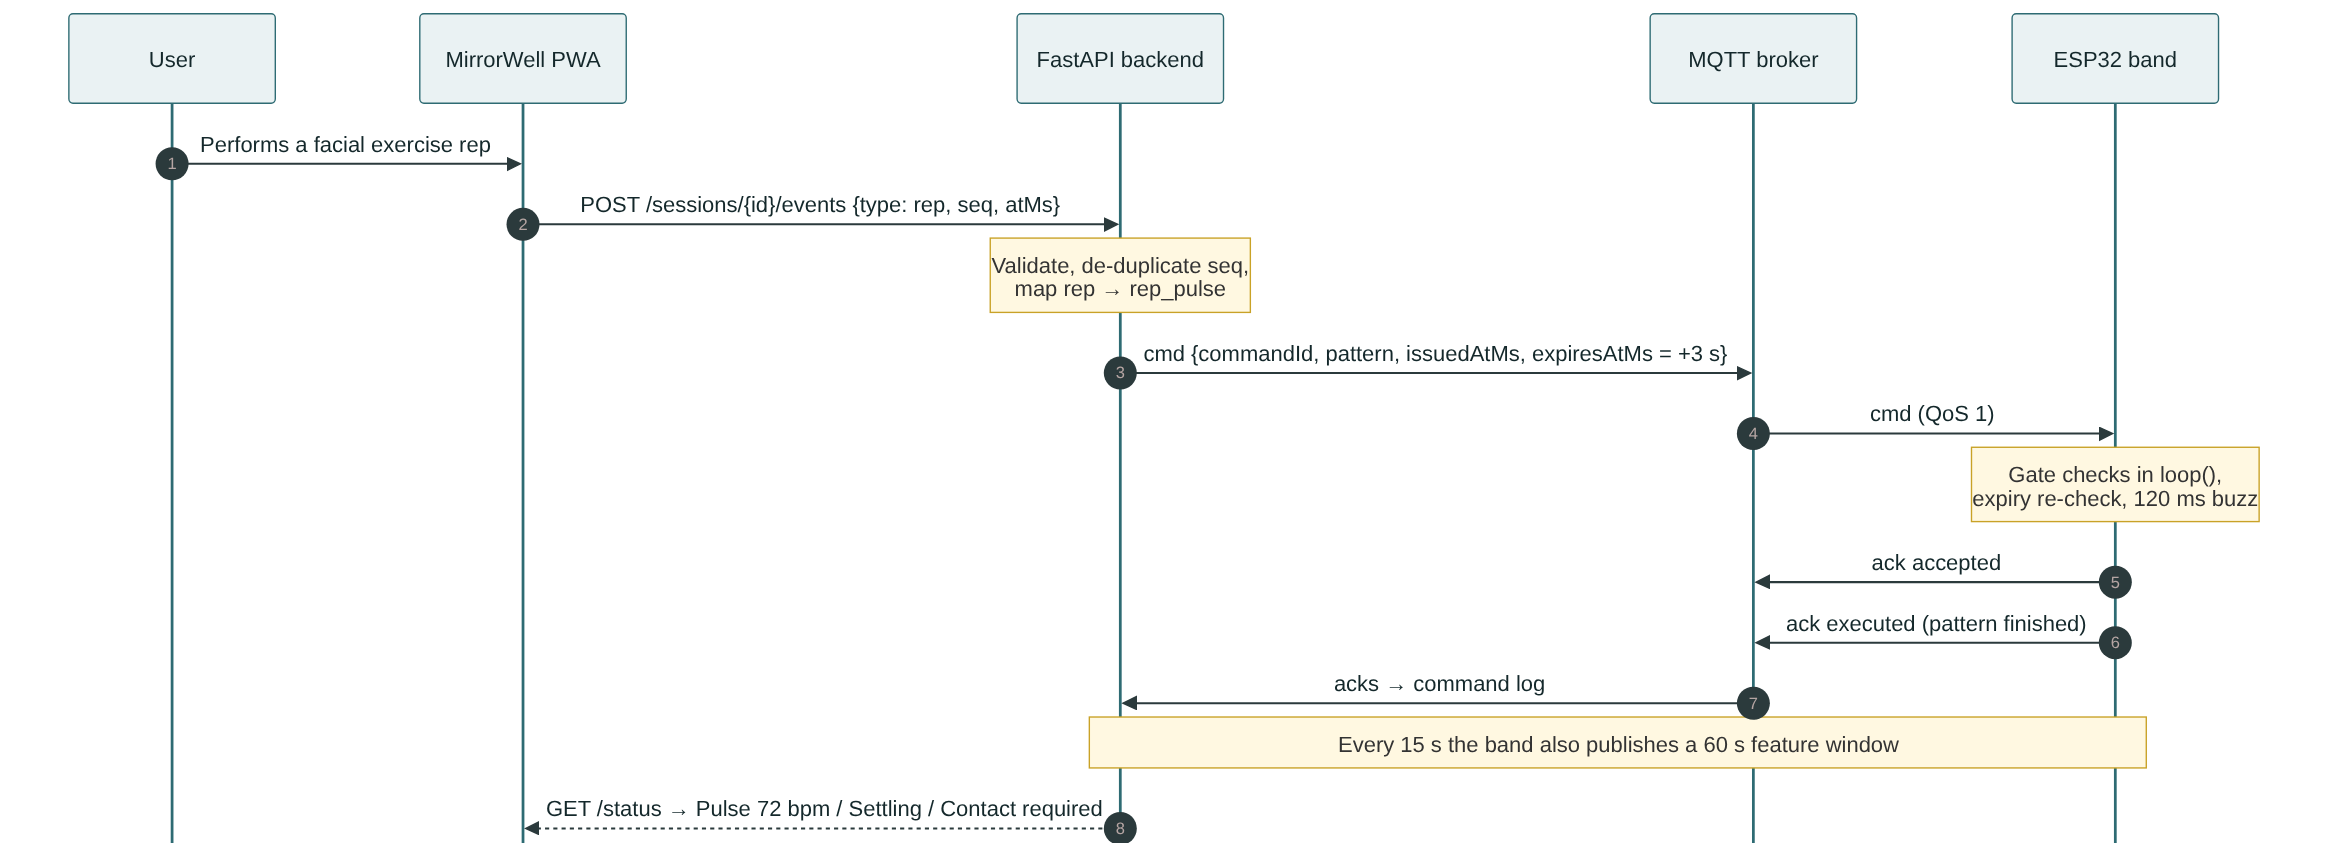
\includegraphics[width=6.3in,height=7.4in,keepaspectratio]{diag_seq.png}\caption{Session Workflow for One Repetition}\label{fig:diag_seq}\end{figure}

A complete session follows the same pattern at a larger scale: the user sits still for about 60–75 seconds so a clean \textbf{before} reading can be taken, performs the exercises with buzz cues, then sits still for another 60–75 seconds after the final buzz for a clean \textbf{after} reading. The backend compares the two.


\section{Technology Stack}\label{sec:3.3}

\begin{table}[H]
\centering\small\setstretch{1.0}
\caption{Technology Stack}\label{tab:technology-stack}
\begin{tabular}{|>{\raggedright\arraybackslash}p{\dimexpr 0.175\linewidth-2\tabcolsep-0.4pt\relax}|>{\raggedright\arraybackslash}p{\dimexpr 0.359\linewidth-2\tabcolsep-0.4pt\relax}|>{\raggedright\arraybackslash}p{\dimexpr 0.436\linewidth-2\tabcolsep-0.4pt\relax}|}
\hline
\rowcolor{headgray}\textbf{Layer} & \textbf{Technology} & \textbf{Why it was chosen} \\ \hline
Microcontroller & ESP32, Arduino-ESP32 core 2.0.17, FreeRTOS & Wi-Fi, TLS and two cores at low cost; FreeRTOS tasks keep sensing apart from networking \\ \hline
Firmware libraries & arduino-mqtt 2.5.2, SparkFun MAX3010x & MQTT with QoS 1 publishing; MAX30102 set-up \\ \hline
Messaging & MQTT 3.1.1, EMQX Cloud, TLS & Light publish/subscribe with delivery guarantees \\ \hline
Backend & Python, FastAPI, paho-mqtt & Simple asynchronous HTTP API and MQTT client \\ \hline
Database & SQLite (demo); Supabase (PostgreSQL) planned & Storage for sessions, events, windows, commands and acknowledgements \\ \hline
Front end & MirrorWell PWA (React, MediaPipe) & Existing application; camera processing stays on the device \\ \hline
Testing & C++ host build, Mosquitto, Python, QEMU & Run the same firmware logic on Linux and on an emulated ESP32 \\ \hline
\end{tabular}
\end{table}

\section{Hardware Design and Physical Layout}\label{sec:3.4}

Early designs placed all electronics on the wrist. This was rejected as heavy and fragile. In the final \textbf{desk-hub layout}, only the sensors and the motor are worn: the ESP32 sits on two 170-hole mini breadboards fixed to a small plate on the desk, connected by 30 cm jumper wires to a foam plate on the wrist strap (motion sensor and motor) and to a velcro loop on the fingertip (pulse sensor). Figure 3.3 shows the complete build and Figure 3.4 shows the three parts in detail. The 3D model was built to the real dimensions of the parts so that it could also serve as an assembly guide.


\begin{figure}[H]\centering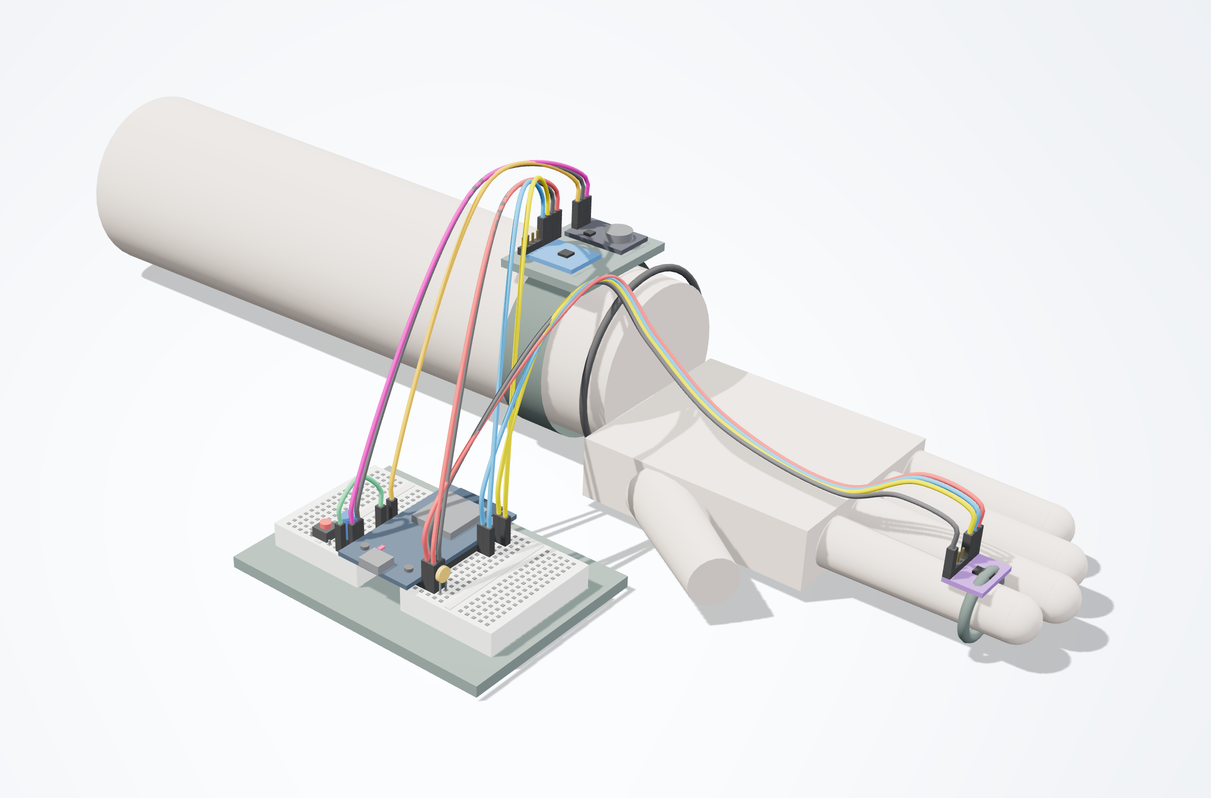
\includegraphics[width=6.0in,height=7.4in,keepaspectratio]{render_hero.png}\caption{3D Render of the Calm Band (Desk Hub, Wrist Strap and Fingertip Sensor)}\label{fig:render_hero}\end{figure}

\begin{figure}[H]\centering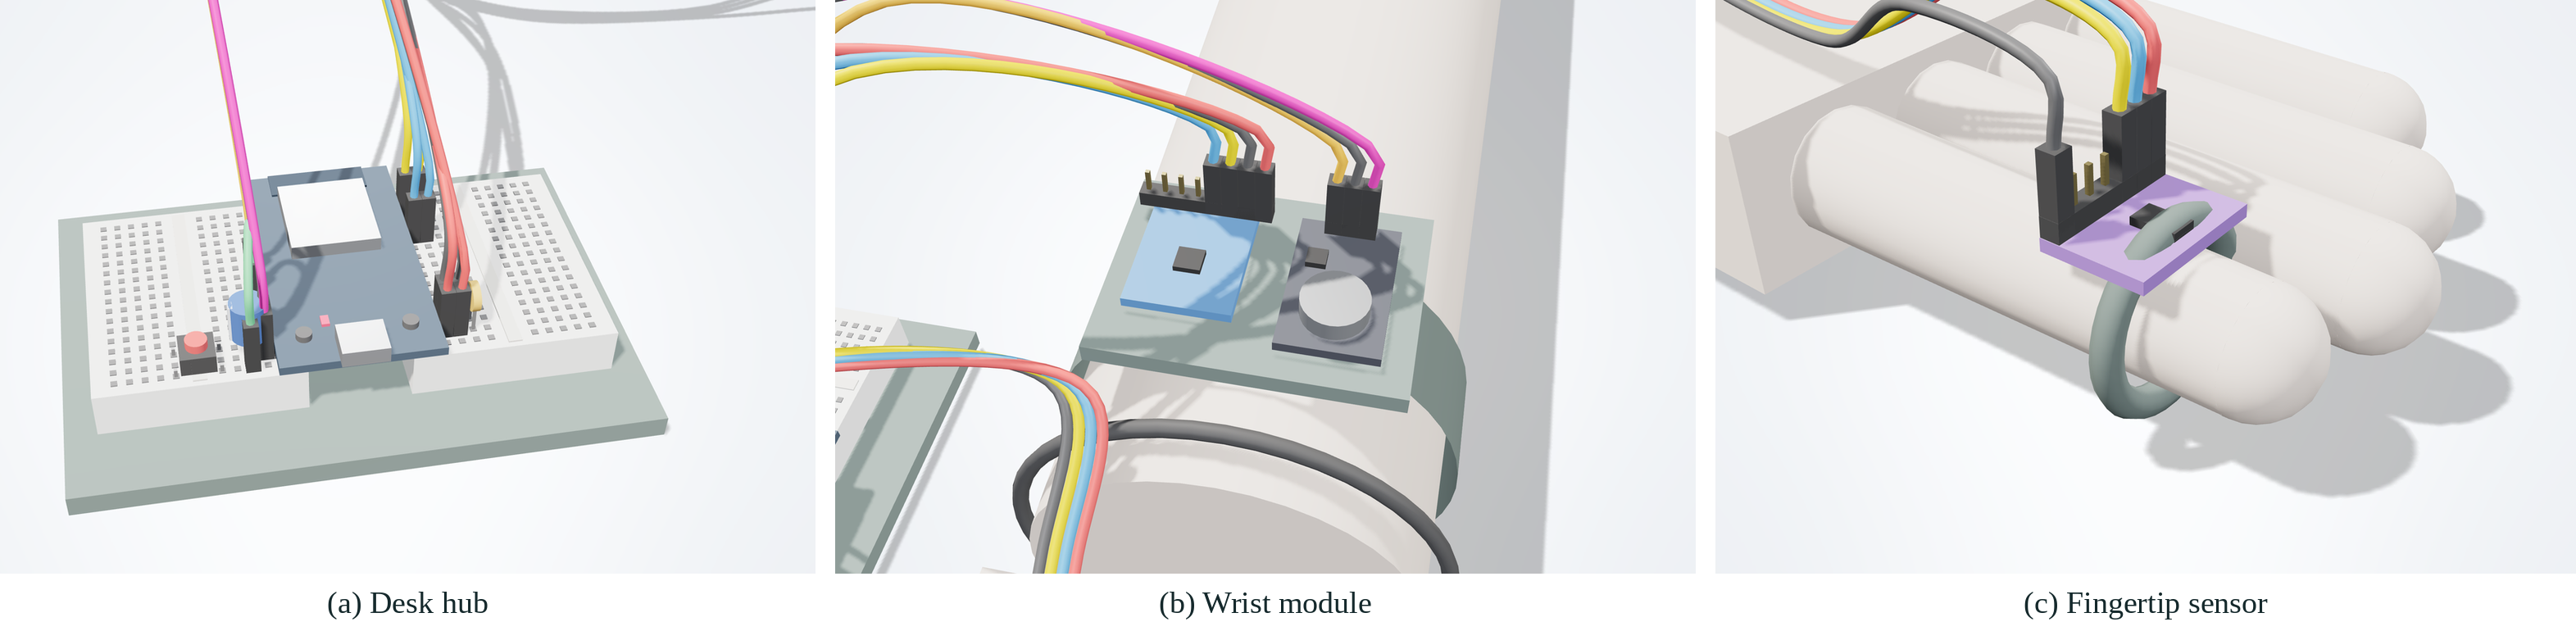
\includegraphics[width=6.3in,height=7.4in,keepaspectratio]{render_closeups.png}\caption{Close-up Renders of the Three Units}\label{fig:render_closeups}\end{figure}

The wiring is shown in Figure 3.5. Both sensors run from the ESP32's 3.3 V regulator; the motor module runs from the 5 V USB supply (VIN) so that its current spikes stay away from the sensor supply. The I²C bus runs at 100 kHz rather than the usual 400 kHz because the 30 cm sensor wires add capacitance. No extra resistors are needed: the sensor boards carry their own pull-up resistors and regulators, the STOP button uses the ESP32's internal pull-up, and the motor module carries its own driver transistor and flyback diode. A 100 µF capacitor across VIN and GND near the motor is recommended to smooth start-up current.


\begin{figure}[H]\centering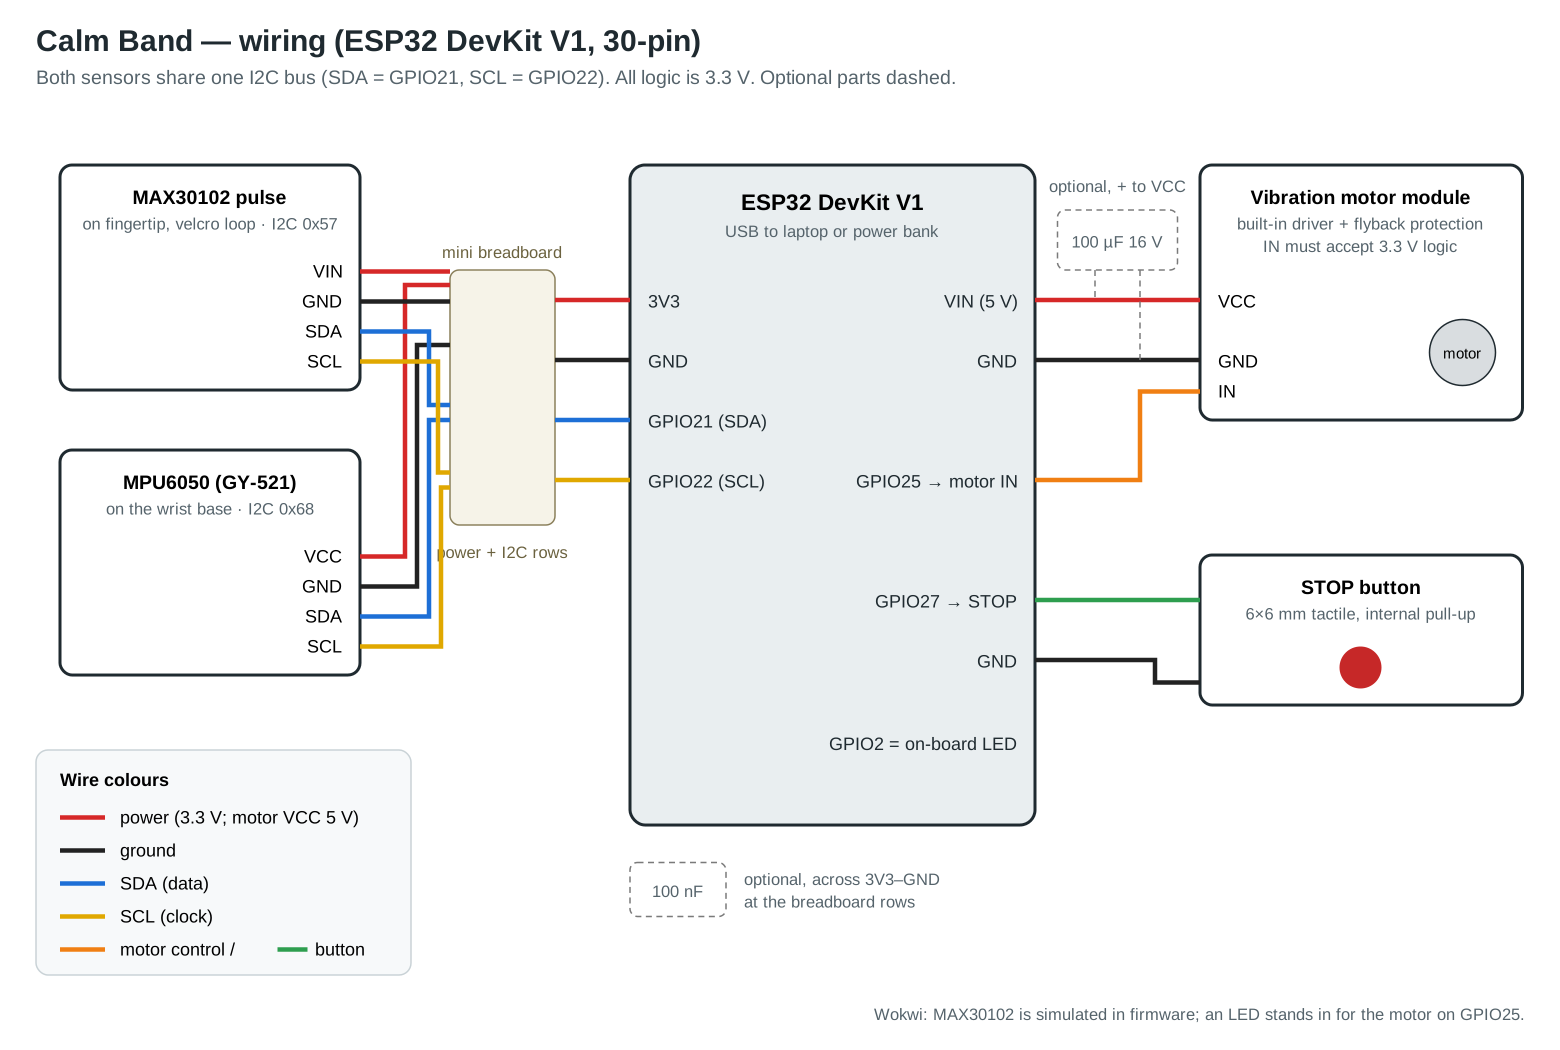
\includegraphics[width=6.3in,height=7.4in,keepaspectratio]{wiring.png}\caption{Wiring Diagram of the Calm Band}\label{fig:wiring}\end{figure}

\begin{table}[H]
\centering\small\setstretch{1.0}
\caption{Pin Assignment on the ESP32}\label{tab:pin-assignment-on-the-esp32}
\begin{tabular}{|>{\raggedright\arraybackslash}p{\dimexpr 0.291\linewidth-2\tabcolsep-0.4pt\relax}|>{\raggedright\arraybackslash}p{\dimexpr 0.320\linewidth-2\tabcolsep-0.4pt\relax}|>{\raggedright\arraybackslash}p{\dimexpr 0.359\linewidth-2\tabcolsep-0.4pt\relax}|}
\hline
\rowcolor{headgray}\textbf{ESP32 pin} & \textbf{Connected to} & \textbf{Notes} \\ \hline
3V3, GND & MAX30102 VIN/GND, MPU6050 VCC/GND & 3.3 V sensor supply \\ \hline
GPIO21 (SDA), GPIO22 (SCL) & Both sensors & Shared I²C bus at 100 kHz \\ \hline
VIN (5 V), GND & Motor module VCC/GND & Separate supply path for the motor \\ \hline
GPIO25 & Motor module IN & Active high, 3.3 V logic \\ \hline
GPIO27 & STOP button to GND & Internal pull-up, falling-edge interrupt, 200 ms debounce \\ \hline
GPIO2 & On-board LED & Connection status \\ \hline
\end{tabular}
\end{table}

\section{Firmware Design}\label{sec:3.5}

The firmware is split into two layers. \texttt{calm\_\allowbreak{}core} contains all the logic (feature windows, beat detection, quality rules, the command gate, vibration patterns, the offline queue and the sensor-health tracker) and has \textbf{no hardware dependencies}, so the identical code runs on the ESP32 and in Linux tests. \texttt{calm\_\allowbreak{}app} is the thin hardware layer: pins, I²C, Wi-Fi, time synchronisation and MQTT.


The firmware uses three independent execution contexts so that a slow network can never disturb sensing or vibration:


\begin{itemize}\item \textbf{Sensor task} (FreeRTOS, core 1, priority above the main loop): wakes every 10 ms, drains the MAX30102's 32-sample hardware buffer directly, reads the MPU6050 once per 32 Hz slot and stamps every sample with its real read time. It never touches the network.
\item \textbf{Motor timer} (\texttt{esp\_\allowbreak{}timer}, every 2 ms): steps the vibration pattern and turns the motor off if it has been on for 1.5 seconds without a break.
\item \textbf{Main loop:} builds feature windows, publishes them, handles queued commands and maintains the MQTT connection. Commands arriving from the network are only copied into a queue inside the MQTT callback and are handled afterwards, because publishing from inside that callback can deadlock the MQTT library.
\end{itemize}

The firmware also has three operating modes. \textbf{LIVE} is normal operation. \textbf{RECORD} (STOP held at power-on) additionally streams the raw 100 Hz pulse signal for building a training dataset. \textbf{BENCH} (no Wi-Fi configured) prints readings to the serial port for testing on the desk.


\section{Backend and Companion Design}\label{sec:3.6}

The backend subscribes to the band's topics, validates every message before it changes any state, stores readings and command acknowledgements, and exposes a small HTTP API to MirrorWell (Table 5.2). It decides the user-facing status with the ordered rules described in Section 4.3. On the MirrorWell side, a companion bridge is enabled only when the application is built with \texttt{VITE\_\allowbreak{}COMPANION\_\allowbreak{}ENABLED=true}. It sends session start, exercise state, repetition and ease-off events and an end-of-session summary to the same origin that served the page, so MirrorWell's no-network rule for the default build is unchanged.


\chapter{METHODOLOGY FOR SENSING, SIGNAL QUALITY AND HAPTIC CUES}\label{ch:4}

\section{Sampling and Feature Windows}\label{sec:4.1}

Sending every raw sample over the network would waste bandwidth and battery and would push all signal processing to the server. Instead, the band summarises its data into \textbf{feature windows}: each window covers the last 60 seconds and a new one is produced every 15 seconds, so consecutive windows overlap by 45 seconds. A 60-second window contains enough heartbeats (typically 60–90) for a stable pulse rate and for later HRV features, while the 15-second step keeps the status reasonably fresh. Table 4.1 lists the parameters.


\begin{table}[H]
\centering\small\setstretch{1.0}
\caption{Sampling and Window Parameters}\label{tab:sampling-and-window-parameters}
\begin{tabular}{|>{\raggedright\arraybackslash}p{\dimexpr 0.272\linewidth-2\tabcolsep-0.4pt\relax}|>{\raggedright\arraybackslash}p{\dimexpr 0.194\linewidth-2\tabcolsep-0.4pt\relax}|>{\raggedright\arraybackslash}p{\dimexpr 0.504\linewidth-2\tabcolsep-0.4pt\relax}|}
\hline
\rowcolor{headgray}\textbf{Parameter} & \textbf{Value} & \textbf{Notes} \\ \hline
Pulse sampling & 100 Hz & MAX30102 at 400 samples/s averaged by 4; IR and red LEDs; 411 µs pulse width \\ \hline
Motion sampling & 32 Hz & MPU6050 at ±2 g (16,384 counts per g) \\ \hline
Window length / step & 60 s / 15 s & 5 s / 1 s in the fast test build \\ \hline
Contact threshold & IR ≥ 50,000 & A window has contact if ≥ 90\% of samples do \\ \hline
Valid beat interval & 300–2,000 ms & Equivalent to 200–30 beats per minute \\ \hline
Minimum valid beats & 20 per window & Otherwise no pulse value is given \\ \hline
Movement threshold & 0.05 g RMS & After gravity is removed per axis \\ \hline
Offline queue & 120 windows & About 30 minutes; oldest dropped first and counted \\ \hline
\end{tabular}
\end{table}

\section{Contact, Pulse and Motion Features}\label{sec:4.2}

\textbf{Contact.} A sample counts as finger contact when its infrared value is at least 50,000; below that the sensor is reading ambient light. A window has contact only when at least 90\% of its samples do.


\textbf{Pulse.} The infrared signal is inverted and its slow baseline is removed. A beat is detected at a local peak that rises above 50\% of a slowly decaying envelope, with at least 300 ms since the previous beat. Each beat-to-beat interval is kept only if it lies between 300 and 2,000 ms. The pulse rate is 60,000 divided by the mean valid interval, in beats per minute. If there is no contact or fewer than 20 valid intervals, the pulse rate is reported as null, never as an estimated or default value.


\textbf{Motion.} For each axis a slow running average (smoothing factor 0.01 at 32 Hz) tracks gravity and is subtracted, so turning the wrist is not mistaken for shaking it. The root mean square (RMS) of what remains is the motion level; the window is marked as moving above 0.05 g. Removing gravity per axis was introduced after testing showed that a sideways arm swing was otherwise under-detected (0.046 g instead of 0.27 g).


\section{Signal Quality and Eligibility Rules}\label{sec:4.3}

Every window carries a quality score and a set of flags so that the receiver can decide whether to trust it. The quality score is the fraction of valid beats, capped at 0.5 when there is no pulse value, when the arm is moving, or when motion data is incomplete. The flags are:


\begin{itemize}\item \textbf{motionValid / motionCoverage:} the share of expected motion samples that actually arrived. Below 80\%, motion fields are null, because a disconnected motion sensor must never look like a perfectly still arm.
\item \textbf{timingGap:} some second inside the window had fewer than 80\% of the expected pulse samples, or samples were known to be lost from the sensor's buffer.
\item \textbf{motorActive:} the motor was on at some point in the window. The vibration itself can disturb the optical signal.
\item \textbf{clockValid:} the band's clock was synchronised. Nothing is published until it is.
\end{itemize}

Because rep cues are frequent, almost every window inside a session overlaps a vibration (Figure 4.1). The project therefore adopts a deliberate policy for Phase 1: readings that overlap a vibration or a finger removal are stored but \textbf{not} shown as pulse values. The comparison pulse comes from the last clean window before the session and the first clean window after it. Once real hardware data is available, the time a buzz actually disturbs the signal will be measured, and in-session windows with a margin around each cue may be used.


\begin{figure}[H]\centering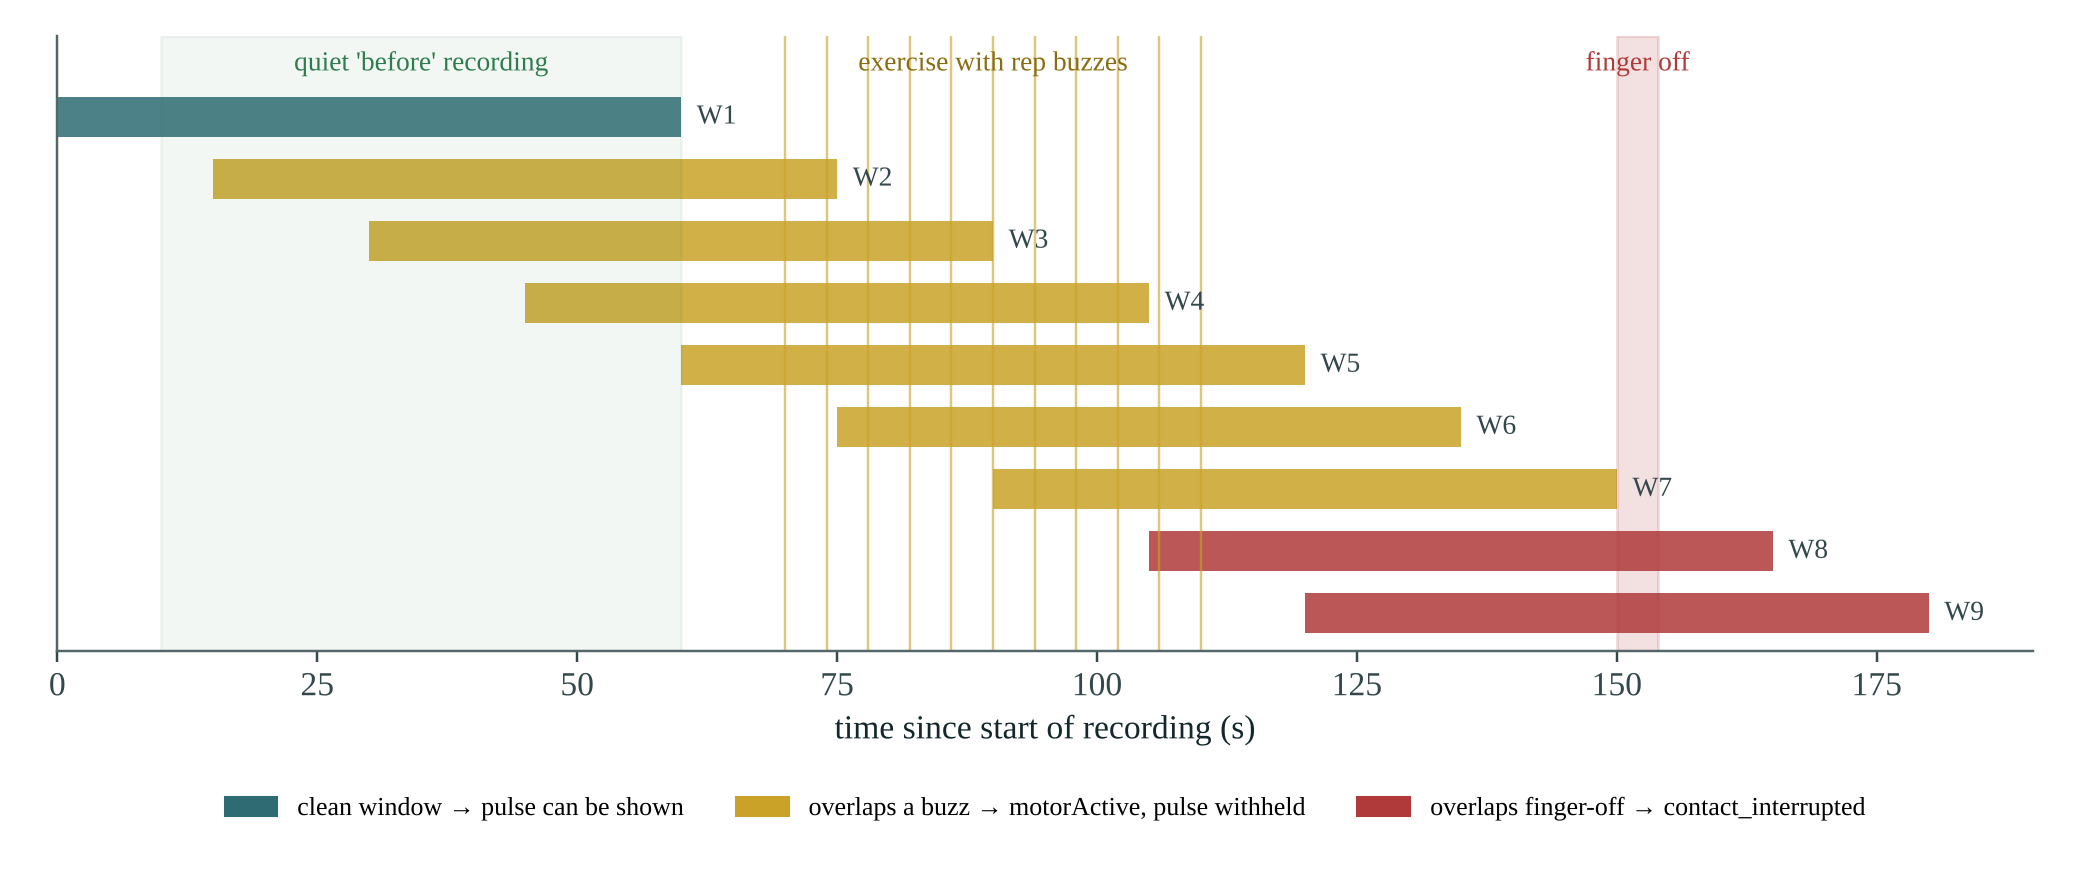
\includegraphics[width=6.3in,height=7.4in,keepaspectratio]{chart_windows.png}\caption{Overlapping Feature Windows and Their Eligibility}\label{fig:chart_windows}\end{figure}

The backend turns these flags into one status for the user, checked in the order shown in Table 4.2; the first matching rule wins. Only the last state shows a pulse value.


\begin{table}[H]
\centering\small\setstretch{1.0}
\caption{Status Rules Applied by the Backend (in order)}\label{tab:status-rules-applied-by-the-backend-in-o}
\begin{tabular}{|>{\raggedright\arraybackslash}p{\dimexpr 0.242\linewidth-2\tabcolsep-0.4pt\relax}|>{\raggedright\arraybackslash}p{\dimexpr 0.728\linewidth-2\tabcolsep-0.4pt\relax}|}
\hline
\rowcolor{headgray}\textbf{State} & \textbf{When it applies} \\ \hline
offline & The band's retained status message says it is offline (clean disconnect or Last Will) \\ \hline
stale & No message from the band for 45 seconds (the backend's own commands do not count) \\ \hline
sensor\_missing & The band reports the pulse or motion sensor as missing \\ \hline
contact\_required & The band's immediate contact signal says the finger is off \\ \hline
collecting & Connected, but no reading yet from the current boot \\ \hline
reading\_stale & The newest reading ended more than 30 seconds ago (by the band's own clock) \\ \hline
settling & The finger is back, but no clean reading has started since it returned \\ \hline
vibration\_overlap & The only problem is that a buzz played during the window \\ \hline
poor\_quality & Quality below 0.8, timing gap, movement or missing motion data \\ \hline
usable & None of the above: the pulse value is shown \\ \hline
\end{tabular}
\end{table}

\section{Command Protocol and Safety Checks}\label{sec:4.4}

Vibration commands are the only way the system acts on the user, so they are checked on the band itself, not only on the backend (Figure 4.2). A command must be a single, flat JSON object with a command identifier, a pattern name and issue and expiry times. It is rejected if it is malformed, has been seen before in this boot, arrives before the clock is set, has inconsistent times (lifetime above 10 seconds or issued more than 2 seconds in the future), has expired or was issued more than 5 seconds ago, or names an unknown pattern or a duration above 1.5 seconds. The expiry is checked once more immediately before the motor starts, with no network operation in between.


\begin{figure}[H]\centering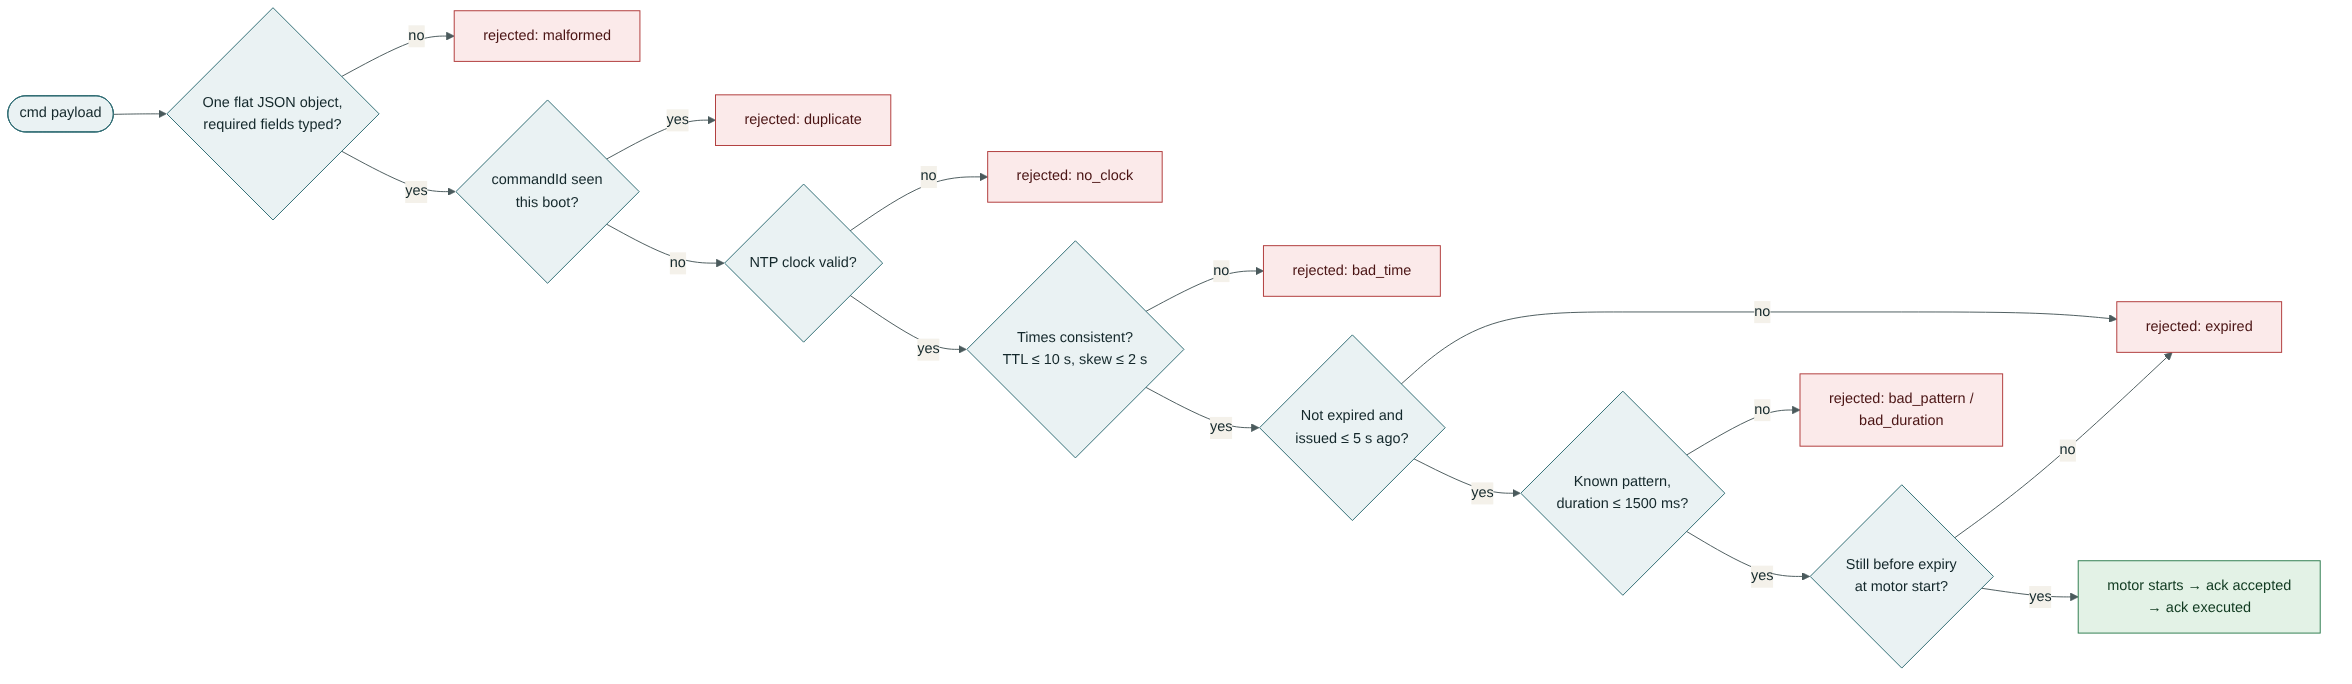
\includegraphics[width=6.3in,height=7.4in,keepaspectratio]{diag_gate.png}\caption{Command Checks on the Band}\label{fig:diag_gate}\end{figure}

\begin{table}[H]
\centering\small\setstretch{1.0}
\caption{Vibration Patterns}\label{tab:vibration-patterns}
\begin{tabular}{|>{\raggedright\arraybackslash}p{\dimexpr 0.194\linewidth-2\tabcolsep-0.4pt\relax}|>{\raggedright\arraybackslash}p{\dimexpr 0.407\linewidth-2\tabcolsep-0.4pt\relax}|>{\raggedright\arraybackslash}p{\dimexpr 0.126\linewidth-2\tabcolsep-0.4pt\relax}|>{\raggedright\arraybackslash}p{\dimexpr 0.242\linewidth-2\tabcolsep-0.4pt\relax}|}
\hline
\rowcolor{headgray}\textbf{Pattern} & \textbf{Motor on/off sequence (ms)} & \textbf{Total} & \textbf{Used for} \\ \hline
rep\_pulse & on 120 & 120 ms & Each completed repetition \\ \hline
ease\_off & on 120, off 100, on 120 & 340 ms & Over-effort detected by MirrorWell \\ \hline
session\_complete & on 300, off 150, on 300, off 150, on 600 & 1,500 ms & End of session \\ \hline
breath\_in & on 80, off 80, on 80 & 240 ms & Guided breathing (Phase 4) \\ \hline
breath\_out & on 400 & 400 ms & Guided breathing (Phase 4) \\ \hline
\end{tabular}
\end{table}

Commands are never retained by the broker and the band connects with a clean session, so a command sent while the band was offline is discarded rather than delivered late. Pressing STOP turns the motor pin off inside the interrupt routine, acknowledges the interrupted command as stopped and reports a button event.


\section{Programming Languages and Libraries Used}\label{sec:4.5}

\begin{itemize}\item \textbf{C++ (Arduino-ESP32 2.0.17, FreeRTOS):} firmware; \texttt{calm\_\allowbreak{}core} is plain C++ with no Arduino dependencies.
\item \textbf{arduino-mqtt 2.5.2} (MQTT client supporting QoS 1 publishing) and \textbf{SparkFun MAX3010x} (sensor set-up). PubSubClient was rejected because it publishes only at QoS 0 and has a 256-byte buffer.
\item \textbf{Python 3 with FastAPI, Uvicorn, paho-mqtt and httpx:} backend and test scripts.
\item \textbf{libmosquitto and Mosquitto:} the Linux build of the band and the local broker used in tests.
\item \textbf{TypeScript and React:} the MirrorWell companion bridge.
\item \textbf{QEMU 9.0 (Espressif build):} running the real ESP32 binary on an emulated chip.
\end{itemize}

\section{Planned Stress Estimation (Machine Learning)}\label{sec:4.6}

Phase 2 adds an experimental calm/tense estimate. The model will be trained on the WESAD dataset [8], using wrist pulse and motion with labels for baseline and amusement (calm) versus the stress test (tense). Models will be compared in increasing complexity: a majority-class baseline, a simple threshold rule, Logistic Regression and Random Forest, reported with accuracy and F1 score. Estimates will be made from the clean before and after windows only, and every unusable window will be labelled unavailable rather than calm. Phase 3 will collect a small pilot dataset with the band in RECORD mode, which now also stores time-matched motion and quality data alongside the raw pulse.


\chapter{IMPLEMENTATION OF THE PROJECT}\label{ch:5}

\section{Firmware Implementation}\label{sec:5.1}

The firmware consists of \texttt{calm\_\allowbreak{}core.h/\allowbreak{}.cpp} (logic), \texttt{calm\_\allowbreak{}app.cpp} (hardware layer), \texttt{config.h} (pins and build switches) and \texttt{secrets.h} (Wi-Fi and broker credentials, not committed). Key implementation details are:


\begin{itemize}\item \textbf{Direct FIFO reading.} The MAX30102 driver keeps only 4 samples in its own buffer, so any delay over 40 ms loses data. The sensor task therefore reads the chip's 32-sample FIFO directly through a small checked-bus interface. The chip's overflow counter is reported as lost samples, which mark the affected windows with a timing gap.
\item \textbf{Sensor health.} Every I²C transaction is checked. Ten failed pulse-sensor reads in a row (about 0.1 s) or 32 failed motion-sensor reads (about 1 s) mark the sensor as missing in the status message; a missing sensor is re-initialised every 5 seconds, and after the pulse sensor recovers no window is clean until a full window has passed.
\item \textbf{Immediate contact events.} A finger on/off signal, debounced over 1 second, is published as soon as it changes, separately from the 60-second windows.
\item \textbf{Offline queue.} While the broker is unreachable, windows are kept in a 120-slot queue and sent oldest first with their original timestamps when the connection returns.
\item \textbf{Strict JSON parser.} Commands are parsed by a small validating parser that rejects truncated text, trailing bytes, nested values, duplicate keys and non-finite numbers.
\end{itemize}

\section{MQTT Interface}\label{sec:5.2}

All messages use the topic prefix \texttt{calmband/\allowbreak{}\textless{}device\textgreater{}/\allowbreak{}}. Table 5.1 lists the topics. Messages from the band use QoS 1, which guarantees at-least-once delivery; duplicates are removed by the backend using the device, boot identifier and sequence number. The status topic is retained and is also the broker's Last Will, so the backend always knows whether the band is online.


\begin{table}[H]
\centering\small\setstretch{1.0}
\caption{MQTT Topics}\label{tab:mqtt-topics}
\begin{tabular}{|>{\raggedright\arraybackslash}p{\dimexpr 0.136\linewidth-2\tabcolsep-0.4pt\relax}|>{\raggedright\arraybackslash}p{\dimexpr 0.194\linewidth-2\tabcolsep-0.4pt\relax}|>{\raggedright\arraybackslash}p{\dimexpr 0.078\linewidth-2\tabcolsep-0.4pt\relax}|>{\raggedright\arraybackslash}p{\dimexpr 0.116\linewidth-2\tabcolsep-0.4pt\relax}|>{\raggedright\arraybackslash}p{\dimexpr 0.446\linewidth-2\tabcolsep-0.4pt\relax}|}
\hline
\rowcolor{headgray}\textbf{Topic} & \textbf{Direction} & \textbf{QoS} & \textbf{Retained} & \textbf{Content} \\ \hline
features & band → backend & 1 & No & Feature window (about 350 bytes) \\ \hline
status & band → backend & 1 & Yes & Online state, sensor health, counters \\ \hline
events & band → backend & 1 & No & STOP pressed; finger contact on/off \\ \hline
cmd & backend → band & 1 & Never & Vibration command with expiry \\ \hline
ack & band → backend & 1 & No & accepted / executed / rejected / stopped \\ \hline
raw & band → recorder & 0 & No & RECORD mode only: raw 100 Hz pulse \\ \hline
\end{tabular}
\end{table}

\section{Backend Implementation}\label{sec:5.3}

The backend is a FastAPI application with an MQTT client running in the background. Its main responsibilities are validation, state, status and command issuing. Every incoming message is parsed, type-checked (including rejecting NaN and infinite numbers) and range-checked inside a single error boundary, so a malformed message is counted and dropped without interrupting reception. Readings are linked to sessions by the band's own timestamps rather than arrival time, so a reading delivered late after an outage still belongs to the right session. Table 5.2 lists the HTTP endpoints.


\begin{table}[H]
\centering\small\setstretch{1.0}
\caption{Backend HTTP Endpoints}\label{tab:backend-http-endpoints}
\begin{tabular}{|>{\raggedright\arraybackslash}p{\dimexpr 0.436\linewidth-2\tabcolsep-0.4pt\relax}|>{\raggedright\arraybackslash}p{\dimexpr 0.533\linewidth-2\tabcolsep-0.4pt\relax}|}
\hline
\rowcolor{headgray}\textbf{Method and path} & \textbf{Purpose} \\ \hline
POST /api/companion/sessions & Open a companion session \\ \hline
POST /api/companion/sessions/\{id\}/events & Exercise state, repetition and ease-off events; returns the command issued \\ \hline
POST /api/companion/sessions/\{id\}/end & End-of-session summary; issues the session\_complete cue \\ \hline
GET /api/companion/status & Current state, pulse (only when usable), contact, sensors and freshness \\ \hline
GET /api/companion/reviewer/sessions & Per-session counts, before/after pulse and command log \\ \hline
\end{tabular}
\end{table}

\section{MirrorWell Companion Bridge}\label{sec:5.4}

The bridge (\texttt{companionBridge.ts}) hooks into MirrorWell's existing session controller events. It sends only an allow-listed set of numbers: session start time, exercise state changes, repetition index and peak effort, ease-off on/off, and an end summary with repetitions completed, mean symmetry and effort indices, ease-off count and the share of low-quality camera frames. It is off by default and is tested by MirrorWell's own unit tests and its no-network end-to-end check, which still passes with the companion both on and off.


\section{Simulation and Test Harness}\label{sec:5.5}

Because the parts were still being ordered, the system was built to be fully testable without hardware:


\begin{itemize}\item \textbf{Core unit tests (48):} run \texttt{calm\_\allowbreak{}core} on Linux, including a fake MAX30102 that follows the datasheet's FIFO behaviour (overflow, partial reads, disconnect and reconnect).
\item \textbf{Simulated band:} a Linux program that runs the same \texttt{calm\_\allowbreak{}core} with a synthetic pulse (about 72 bpm with slow drift) and synthetic motion over a real MQTT connection. Test hooks can remove the finger, shake the arm, press STOP, drop the network, invalidate the clock or disconnect the motion sensor.
\item \textbf{Backend status checks (33):} inject messages directly to test every status rule, broken messages and late deliveries.
\item \textbf{Integration checks (13) and firmware scenarios (23):} run the simulated band, broker and backend together end to end.
\item \textbf{One command:} \texttt{run\_\allowbreak{}all\_\allowbreak{}tests.sh} runs all four suites and passes only if every process exits cleanly, no check fails, no exception occurs and the exact expected number of checks ran.
\end{itemize}

\section{Iterative Review and Hardening}\label{sec:5.6}

The implementation was reviewed by an independent validation agent in four rounds. Each round reproduced its findings, and each fix came with a test that failed on the previous version and passed on the new one. Table 5.3 summarises the most important findings.


\begin{table}[H]
\centering\small\setstretch{1.0}
\caption{Main Findings from the Review Rounds}\label{tab:main-findings-from-the-review-rounds}
\begin{tabular}{|>{\raggedright\arraybackslash}p{\dimexpr 0.097\linewidth-2\tabcolsep-0.4pt\relax}|>{\raggedright\arraybackslash}p{\dimexpr 0.466\linewidth-2\tabcolsep-0.4pt\relax}|>{\raggedright\arraybackslash}p{\dimexpr 0.407\linewidth-2\tabcolsep-0.4pt\relax}|}
\hline
\rowcolor{headgray}\textbf{Round} & \textbf{Finding} & \textbf{Fix} \\ \hline
1 & Acknowledgements were published inside the MQTT callback (deadlock risk) & Commands queued in the callback, handled in the main loop \\ \hline
1 & The 1.5 s motor limit depended on the network loop & Motor driven by a 2 ms timer with a continuous-on cut-off \\ \hline
1 & A missing motion sensor looked like a perfectly still arm & Motion coverage and validity flags; null motion fields \\ \hline
1 & Old or our own messages kept a reading 'usable' & Connectivity and freshness separated; offline status honoured \\ \hline
2 & Sensor reads shared the network loop; driver buffer could overflow & Dedicated sensor task; direct FIFO reads; lost samples flagged \\ \hline
2 & A previous boot's reading appeared current & Status uses the current boot only \\ \hline
3 & Wrong-type and NaN values crashed or polluted the backend & Type-first validation, finite numbers only, one error boundary \\ \hline
3 & Pulse sensor never recovered after a failure & Checked reads, health tracking, retries, clean-window rule \\ \hline
4 & Old pulse returned after a brief finger removal & Finger-off periods tracked; reading must start after contact returns \\ \hline
\end{tabular}
\end{table}

\chapter{RESULTS AND DISCUSSION}\label{ch:6}

\section{Test Results}\label{sec:6.1}

All four automated suites pass. Table 6.1 lists the final results, re-run on 26 October 2026 at commit 29d8ad9, and Figure 6.1 shows how the test coverage grew through the review rounds, from 47 checks in the first package to 117.


\begin{table}[H]
\centering\small\setstretch{1.0}
\caption{Automated Test Results}\label{tab:automated-test-results}
\begin{tabular}{|>{\raggedright\arraybackslash}p{\dimexpr 0.213\linewidth-2\tabcolsep-0.4pt\relax}|>{\raggedright\arraybackslash}p{\dimexpr 0.582\linewidth-2\tabcolsep-0.4pt\relax}|>{\raggedright\arraybackslash}p{\dimexpr 0.175\linewidth-2\tabcolsep-0.4pt\relax}|}
\hline
\rowcolor{headgray}\textbf{Suite} & \textbf{What it covers} & \textbf{Result} \\ \hline
Core unit tests & Windows, beats, motion, quality, command gate, patterns, outbox, FIFO reader, sensor health, contact & 48 / 48 \\ \hline
Backend status checks & Every status rule, malformed and wrong-type messages, late delivery, finger removal & 33 / 33 \\ \hline
Integration & Simulated band ↔ broker ↔ backend: sessions, cues, duplicates, expiry & 13 / 13 \\ \hline
Firmware scenarios & Movement, contact loss, STOP, motor flag, clock loss, network drop, broken commands, sensor loss & 23 / 23 \\ \hline
\rowcolor{totalgray}\textbf{Total} & \textbf{} & \textbf{117 / 117} \\ \hline
\end{tabular}
\end{table}

\begin{figure}[H]\centering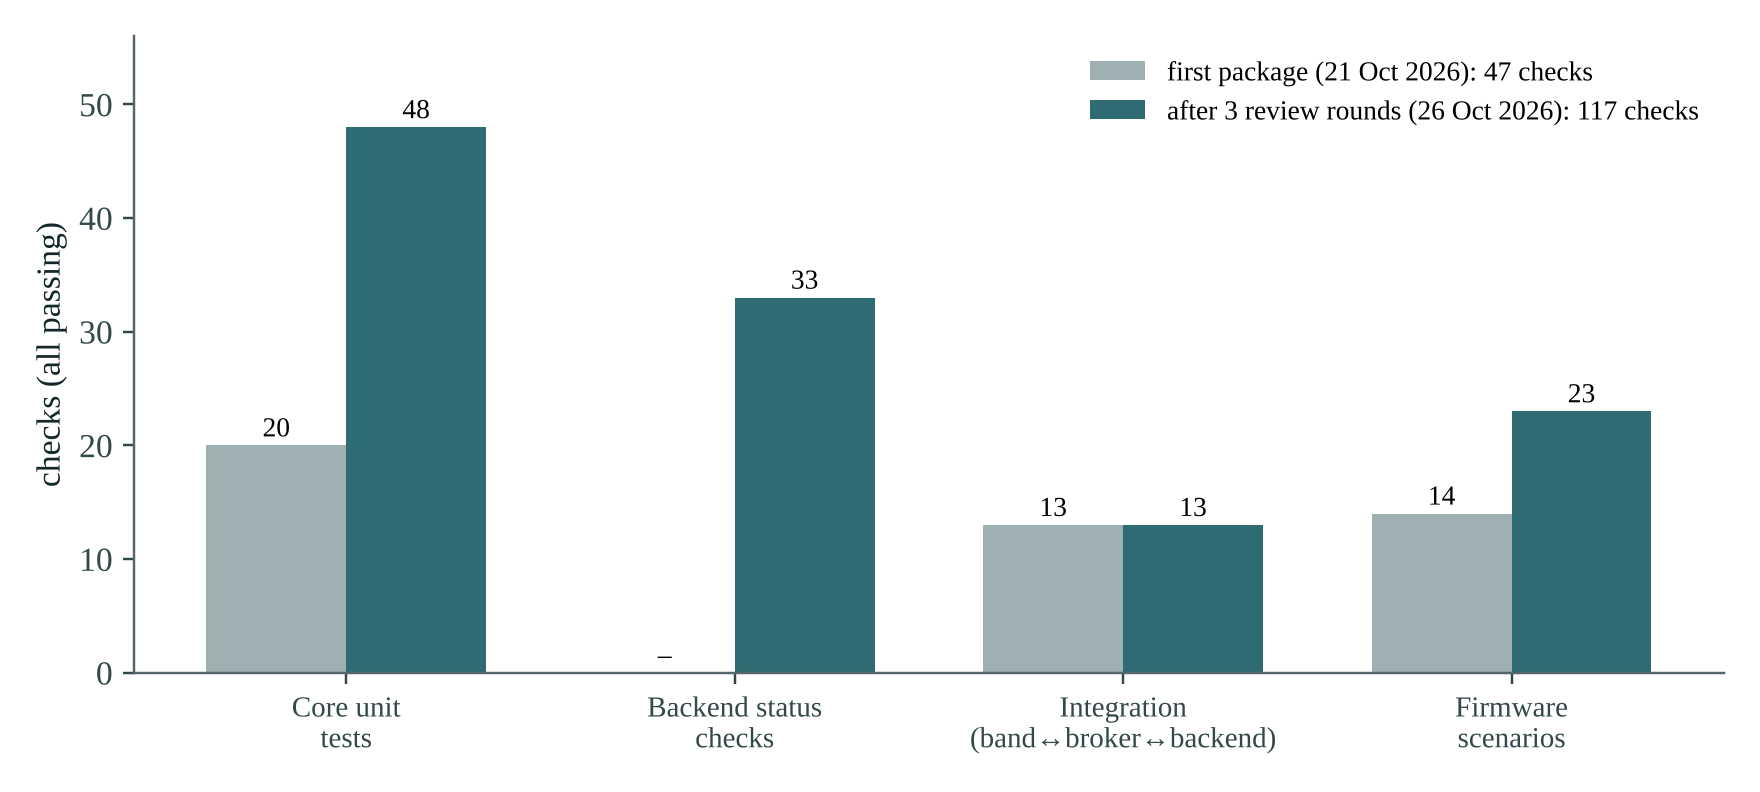
\includegraphics[width=5.8in,height=7.4in,keepaspectratio]{chart_tests.png}\caption{Growth of the Automated Test Suites}\label{fig:chart_tests}\end{figure}

\section{Resource Usage on the ESP32}\label{sec:6.2}

The firmware was compiled for the ESP32 with the Arduino-ESP32 core 2.0.17. Both builds use 69\% of the 1.3 MB application flash and 35\% of the dynamic memory, leaving ample room for Phase 2–7 features (Table 6.2).


\begin{table}[H]
\centering\small\setstretch{1.0}
\caption{Firmware Size}\label{tab:firmware-size}
\begin{tabular}{|>{\raggedright\arraybackslash}p{\dimexpr 0.427\linewidth-2\tabcolsep-0.4pt\relax}|>{\raggedright\arraybackslash}p{\dimexpr 0.272\linewidth-2\tabcolsep-0.4pt\relax}|>{\raggedright\arraybackslash}p{\dimexpr 0.272\linewidth-2\tabcolsep-0.4pt\relax}|}
\hline
\rowcolor{headgray}\textbf{Build} & \textbf{Flash used} & \textbf{RAM used} \\ \hline
Real sensors (MAX30102 + MPU6050) & 913,509 bytes (69\%) & 116,076 bytes (35\%) \\ \hline
Simulated pulse (Wokwi) & 914,781 bytes (69\%) & 116,028 bytes (35\%) \\ \hline
\end{tabular}
\end{table}

\section{Emulated-Hardware Results}\label{sec:6.3}

The real ESP32 binary was run on an emulated ESP32 (Espressif QEMU 9.0.0). In BENCH mode it booted and printed one feature window per second in the fast test build, with no timing gaps. Because the emulator has no motion sensor, every window correctly reported \texttt{motionValid:false} with the quality capped at 0.5; before the review fixes, the same situation was wrongly reported as quality 1.0.


Two self-tests were also run on the emulated chip, each blocking the main loop for 3 seconds as a stuck network call would. In the \textbf{motor self-test} (Figure 6.2) the longest pattern ran with all six on/off edges and the motor turned off at +1,500 ms; in an earlier run it was +1,503 ms, so the limit should be read as within a few milliseconds rather than exact. In the \textbf{sensor self-test}, the sensor task produced 301 of about 300 expected pulse samples and ran all 96 motion read slots on time, with none missed or lost. These results show that sensing and vibration timing are independent of the network loop. They do not test the physical sensors, because the emulator's pulse signal is synthetic and it has no motion sensor.


\begin{figure}[H]\centering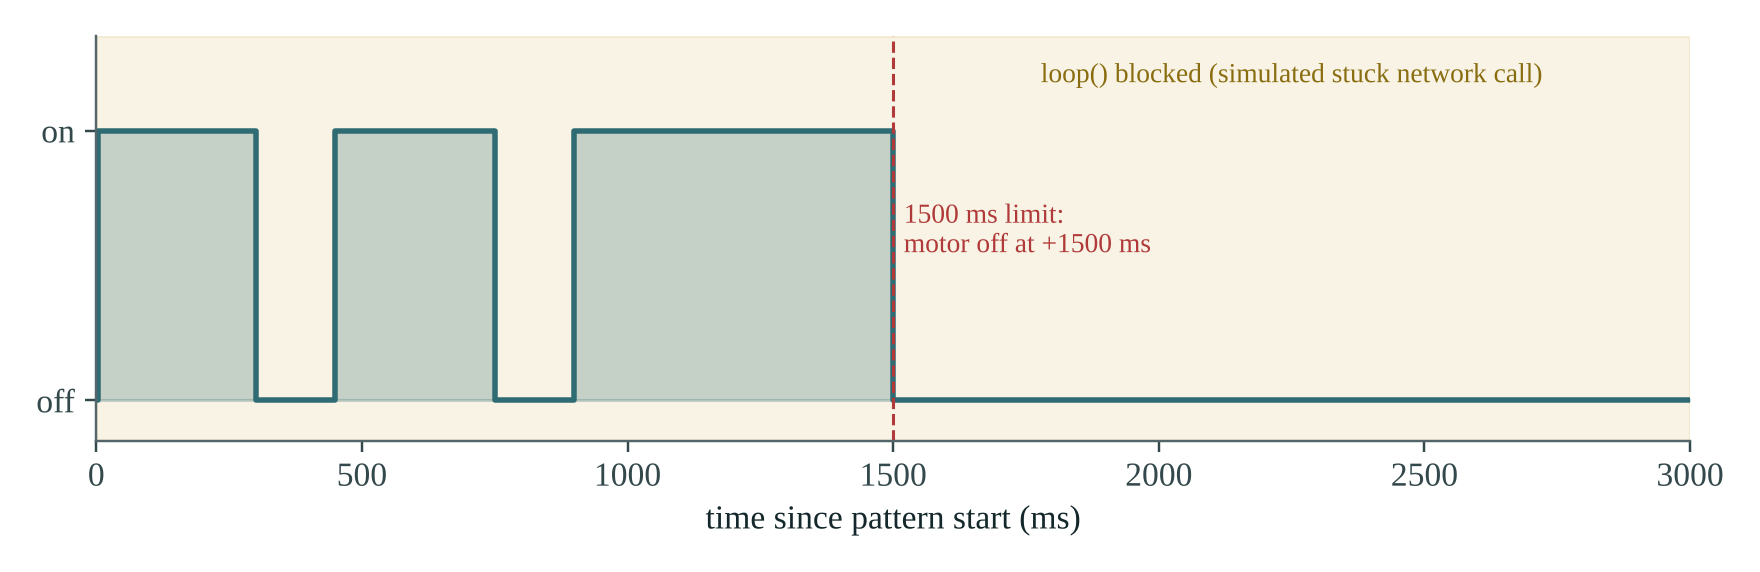
\includegraphics[width=6.0in,height=7.4in,keepaspectratio]{chart_selftest.png}\caption{Motor Self-Test on the Emulated ESP32}\label{fig:chart_selftest}\end{figure}

\section{Real Hardware Results}\label{sec:6.hw}

After the parts arrived, the hub was assembled on two breadboards with the delivered components: an ESP32 DevKit V1 (30-pin, CP2102 USB bridge), a MAX30102 breakout (HW-605), a GY-521 motion board and a vibration motor module with a built-in driver. It was tested in three stages on 15 and 16 November 2026: part-by-part bring-up, the full firmware in BENCH mode (no network), and the complete online chain with MirrorWell. The wiring followed Table~\ref{tab:pin-assignment-on-the-esp32}; no firmware logic, safety rule or message format was changed for these tests. The real-sensor build used 913,625 bytes of flash (69\%) and 116,084 bytes of RAM (35\%), matching Table 6.2.

\textbf{Bring-up.} Each part was first checked on its own with a small test sketch (Table~\ref{tab:hardware-bring-up-checks}). Both sensors answered on the shared I²C bus. The motion board's chip reported the identity 0x70, which means it is an MPU-6500-compatible part rather than a genuine MPU6050; it uses the same registers, and the firmware does not check the identity, so it worked unchanged. The motor module ran from the 3.3 V GPIO25 signal with its supply on VIN (5 V), confirming the assumption flagged in Section~\ref{sec:6.5}.

\begin{table}[H]
\centering\small\setstretch{1.0}
\caption{Hardware Bring-up Checks}\label{tab:hardware-bring-up-checks}
\begin{tabular}{|>{\raggedright\arraybackslash}p{\dimexpr 0.24\linewidth-2\tabcolsep-0.4pt\relax}|>{\raggedright\arraybackslash}p{\dimexpr 0.50\linewidth-2\tabcolsep-0.4pt\relax}|>{\raggedright\arraybackslash}p{\dimexpr 0.26\linewidth-2\tabcolsep-0.4pt\relax}|}
\hline
\rowcolor{headgray}\textbf{Part} & \textbf{Check} & \textbf{Result} \\ \hline
Vibration motor & IN on GPIO25, VCC on VIN (5 V), GND & Buzzes \\ \hline
STOP button & GPIO27 to GND, pressed during a pattern & Motor cut immediately \\ \hline
MAX30102 & I²C scan (SDA GPIO21, SCL GPIO22) & Found at 0x57 \\ \hline
Motion board (GY-521) & I²C scan; identity register; acceleration at rest & Found at 0x68; ID 0x70 (MPU-6500 compatible); |a| ≈ 1.02 g \\ \hline
\end{tabular}
\end{table}

\textbf{BENCH mode.} With the full firmware and no Wi-Fi configured, the band printed its feature windows to the serial port. Table~\ref{tab:bench-mode-pulse-readings} shows five consecutive windows with a fingertip resting still on the sensor. Quality stayed at 0.98–1.00 and the spread of the beat-to-beat rate fell from 34.7 to 6.0 BPM as the finger settled, while the number of valid beat intervals rose from 78 to 100. When the finger was moving or unsteady, the pulse was correctly reported as \texttt{null} (only 1–6 valid intervals, below the minimum of 20) and the window was marked \texttt{moving} at a peak of 1.3 g, which is the intended safety behaviour.

\begin{table}[H]
\centering\small\setstretch{1.0}
\caption{BENCH-Mode Pulse Readings with a Still Fingertip}\label{tab:bench-mode-pulse-readings}
\begin{tabular}{|c|c|c|c|c|}
\hline
\rowcolor{headgray}\textbf{Window} & \textbf{Quality} & \textbf{Pulse (BPM)} & \textbf{Spread, SD (BPM)} & \textbf{Valid beat intervals} \\ \hline
1 & 0.98 & 102.9 & 34.7 & 78 \\ \hline
2 & 0.98 & 98.1 & 17.4 & 86 \\ \hline
3 & 0.99 & 99.4 & 7.1 & 94 \\ \hline
4 & 0.99 & 99.4 & 7.3 & 95 \\ \hline
5 & 1.00 & 100.9 & 6.0 & 100 \\ \hline
\end{tabular}
\end{table}

\textbf{End-to-end test.} The complete chain was then run online: band $\rightarrow$ phone hotspot (2.4 GHz) $\rightarrow$ Mosquitto 2.1.2 broker on a Windows laptop $\rightarrow$ FastAPI backend $\rightarrow$ MirrorWell in Chrome. For this test the broker was local, with plain MQTT on port 1883 rather than TLS. Table~\ref{tab:end-to-end-results-real-hardware} lists the results; all checks passed.

\begin{table}[H]
\centering\small\setstretch{1.0}
\caption{End-to-End Results on the Real Hardware}\label{tab:end-to-end-results-real-hardware}
\begin{tabular}{|>{\raggedright\arraybackslash}p{\dimexpr 0.26\linewidth-2\tabcolsep-0.4pt\relax}|>{\raggedright\arraybackslash}p{\dimexpr 0.60\linewidth-2\tabcolsep-0.4pt\relax}|>{\raggedright\arraybackslash}p{\dimexpr 0.14\linewidth-2\tabcolsep-0.4pt\relax}|}
\hline
\rowcolor{headgray}\textbf{Test} & \textbf{Observed} & \textbf{Result} \\ \hline
Connection & Band joined the hotspot, synchronised its clock over NTP and connected to the broker; both sensors reported ok & Pass \\ \hline
Status, finger still & \texttt{usable}, 97–98 BPM, quality 1.00, 97 valid intervals, motion 0.02 g RMS & Pass \\ \hline
Test vibration command & \texttt{rep\_pulse} and \texttt{ease\_off} acknowledged \texttt{accepted} then \texttt{executed} within about 0.2 s; duration capped at 1,500 ms & Pass \\ \hline
MirrorWell session & Eye-closure exercise, 5 repetitions: 6 of 6 commands executed (5 rep cues and 1 session-complete cue) & Pass \\ \hline
Finger removed & \texttt{contact\_required}, pulse withheld & Pass \\ \hline
Band shaken & \texttt{poor\_quality} (low quality, moving), pulse withheld & Pass \\ \hline
10-minute soak & 40 of 40 windows received in order, 0 timing gaps, 0 rejected messages; 7 repeated deliveries discarded by the backend & Pass \\ \hline
Hotspot interruption & Link lost for about 85 s; band reconnected by itself and re-sent its queued windows (13 failed sends, 0 windows dropped); backend showed the band offline meanwhile & Pass \\ \hline
\end{tabular}
\end{table}

\textbf{Observations.} Two findings came only from the real parts. First, when the pulse sensor was left face-down on a table with no finger on it, the table reflected enough infrared light to pass the contact threshold (raw IR ≥ 50,000), and the band reported a false pulse of 135–151 BPM. The beat-to-beat spread of these readings was very high (29–39 BPM, against about 6–15 BPM for a real finger), and on one occasion the backend showed the false value as usable. With the sensor face-up and uncovered, the band correctly reported no contact. For the demonstration the sensor is kept face-up; a stricter plausibility check is listed as future work. Second, the measured resting pulse of about 98–100 BPM has not yet been compared with a manual pulse count; an earlier simple test sketch read 72–86 BPM on the same sensor.

\section{Data Storage in the Backend}\label{sec:6.store}

The first version of the backend kept everything in memory, so a restart lost every session. The demonstration build stores its data in \textbf{SQLite}, a file-based database that needs no separate server and is used through Python's standard library. The database has seven tables: \texttt{meta}, \texttt{sessions} (start, end and state), \texttt{session\_events} (the MirrorWell events), \texttt{windows} (the feature windows, each with its \texttt{origin}), \texttt{band\_events} (every finger-contact and button event), \texttt{commands} and \texttt{acks} (every vibration command and each acknowledgement the band sent for it).

The duplicate rules did not change: a window is identified by device, boot and sequence number, and a MirrorWell event by session and sequence number, so a repeated delivery is stored once. After a restart the backend reloads the history, rebuilds the finger-off periods from the stored contact events and restores the active session. The live status rules still use only the current boot of the band, so old data never makes a new reading look current.

The file location is set by the \texttt{CALMBAND\_DB} variable. The simulated band and the real demonstration use \emph{separate} databases (\texttt{calmband-sim.db} and \texttt{calmband-demo.db}), so simulated data can never appear in the demonstration history; the start script for the demo can also rename the demo database with a timestamp to begin from a clean state. Database files are excluded from version control.

\section{Live Band Card in MirrorWell}\label{sec:6.live}

During a session MirrorWell shows a small card beside the camera view. It asks the backend for the band's state every 2 seconds, only while the session screen is open and the companion is switched on, and never in the demonstration mode that uses no band. The card gives sensor feedback \textbf{without showing any raw number}: the person exercising never sees a pulse value. It uses five simple signals instead (Figure~\ref{fig:ui_live_cue}):
\begin{itemize}\item a \textbf{heart} that beats at the measured pace (the interval between beats is sent, not the rate);
\item \textbf{signal bars}, from zero to three, showing how clear the sensor signal is;
\item \textbf{steadiness}, which says ``Steady'' or ``Hold still'' according to the wrist motion sensor;
\item a \textbf{settling arrow} (falling, level or rising) that compares the recent pulse with the start of the session; and
\item a \textbf{cue pulse}, a short flash when the band has just buzzed.
\end{itemize}

\textbf{Measured during wrist cues.} A repetition cue buzzes the band every few seconds, so most 60-second windows overlap a buzz. Such windows are withheld from every summary and index (Chapter~4), but the live card may still show the heart for them, because it is only feedback. When it does, the card prints the words ``measured during wrist cues'' under the heart, so the person can tell it apart from a clean reading. A backend setting can turn this off, in which case the heart is hidden while the band buzzes.

\begin{figure}[H]\centering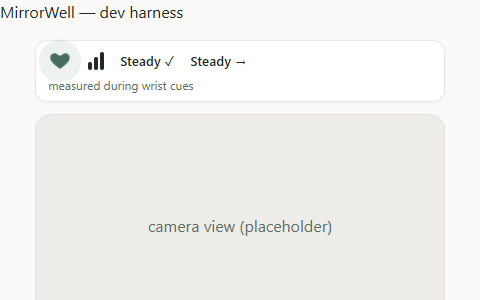
\includegraphics[width=3.2in,height=2.2in,keepaspectratio]{integrated-live-card-during-cue.png}\caption{Live Band Card Showing the Heart, Signal Bars and Steadiness During a Cue}\label{fig:ui_live_cue}\end{figure}

\textbf{Honest ``why'' messages.} When the data is poor, the card says so in plain words instead of showing a stale or invented value (Table~\ref{tab:live-card-messages}, Figures~\ref{fig:ui_live_moving} and~\ref{fig:ui_live_contact}). The heart is greyed out and the signal bars drop. A missing value is never drawn as a calm one.

\begin{table}[H]
\centering\small\setstretch{1.0}
\caption{Messages Shown on the Live Card}\label{tab:live-card-messages}
\begin{tabular}{|>{\raggedright\arraybackslash}p{\dimexpr 0.26\linewidth-2\tabcolsep-0.4pt\relax}|>{\raggedright\arraybackslash}p{\dimexpr 0.74\linewidth-2\tabcolsep-0.4pt\relax}|}
\hline
\rowcolor{headgray}\textbf{State} & \textbf{Message} \\ \hline
\texttt{offline} & The band is off or out of range. \\ \hline
\texttt{sensor\_missing} & A band sensor is not responding. Check its wires. \\ \hline
\texttt{collecting} & Getting a first reading. Rest your fingertip on the sensor and keep still for about a minute. \\ \hline
\texttt{contact\_required} & Rest your fingertip lightly on the sensor. \\ \hline
\texttt{poor\_quality} (moving) & Keep your hand still for a clearer reading. \\ \hline
\texttt{poor\_quality} (other) & The reading is not clear yet. Keep your fingertip still and relaxed on the sensor. \\ \hline
\texttt{usable} & No message; the heart beats \\ \hline
\end{tabular}
\end{table}

\begin{figure}[H]\centering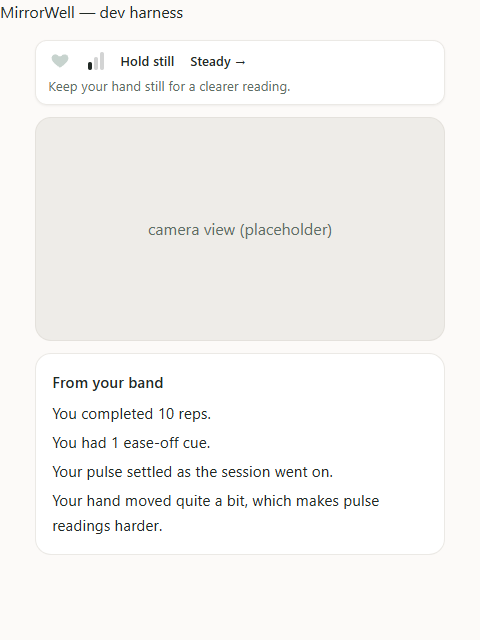
\includegraphics[width=2.6in,height=3.3in,keepaspectratio]{ui-live-poor-quality-moving.png}\caption{Live Card When the Hand Is Moving}\label{fig:ui_live_moving}\end{figure}

\begin{figure}[H]\centering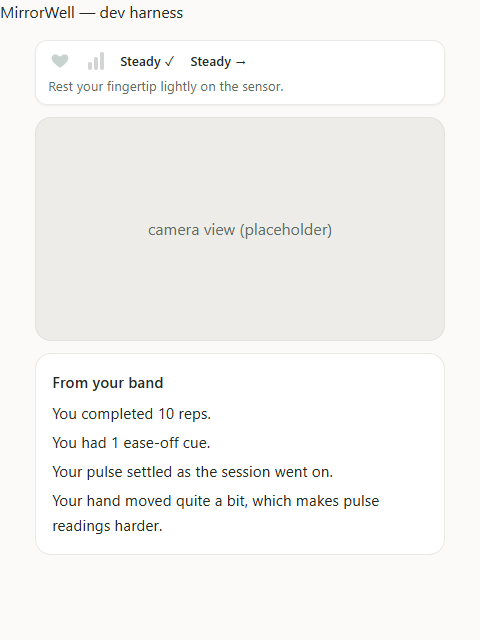
\includegraphics[width=2.6in,height=3.3in,keepaspectratio]{ui-live-contact-required.png}\caption{Live Card When the Finger Is Off the Sensor}\label{fig:ui_live_contact}\end{figure}

\section{Post-Session Summary in Plain Words}\label{sec:6.summary}

When a session ends, MirrorWell shows a short summary headed ``From your band'' (Figure~\ref{fig:ui_summary}). The backend writes the sentences, so the wording lives in one place. Each sentence follows a fixed rule: the number of repetitions and ease-off cues; whether the pulse \emph{settled}, stayed about the same or was a little higher at the end; and whether the hand stayed steady for most of the session. The summary contains no pulse numbers and no index, and it never uses words such as stress, anxiety or diagnosis.

The summary \textbf{waits for the clean reading after the session}. The last 60-second window of a session usually overlaps a buzz, so it cannot be used. The first clean window after the session arrives only 60 to 75 seconds after the end. MirrorWell therefore asks again every few seconds, for up to 180 seconds, until the pulse comparison is available. Until then it shows ``waiting''; if no clean reading ever arrives, it says honestly that the band could not get a clear enough pulse reading this time, rather than guessing.

\begin{figure}[H]\centering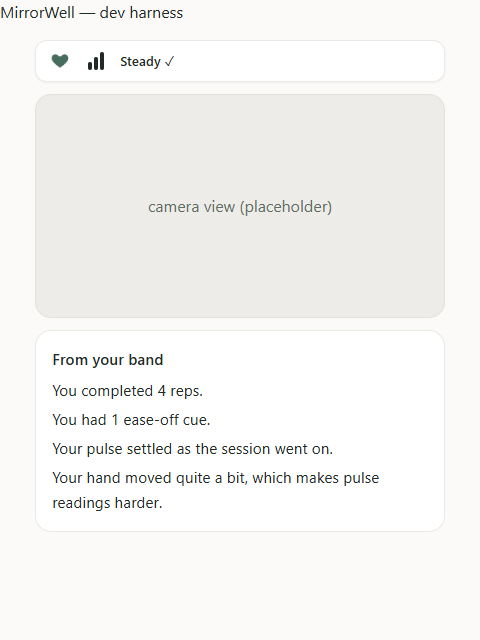
\includegraphics[width=2.6in,height=3.3in,keepaspectratio]{integrated-summary.png}\caption{Post-Session Summary in Plain Words}\label{fig:ui_summary}\end{figure}

\section{Reviewer and Therapist Page}\label{sec:6.reviewer}

A separate page, served by the backend at \texttt{/reviewer/}, is meant for a therapist or reviewer. It uses the same origin as the backend, with no external script, font or chart library. Unlike MirrorWell, it may show pulse values, and it always shows where they came from. It has three parts:
\begin{itemize}\item a \textbf{session list} (Figure~\ref{fig:rev_list}) with date, duration, repetitions, ease-off cues, cues, signal share and mean usable pulse;
\item a \textbf{session timeline} (Figure~\ref{fig:rev_timeline}) drawing the usable pulse as a line that \emph{breaks} wherever there is no usable reading, so gaps are left empty and never joined or filled. Hand movement is shaded, periods when the motor was on are hatched, and a strip underneath colours each window by signal quality. Markers show repetitions, cues (green when executed, red when stopped or rejected, grey when not confirmed), ease-off cues and presses of the STOP button; and
\item \textbf{trends}: sessions per day and the mean usable pulse of each session.
\end{itemize}
Every session carries a \textbf{SIMULATED} badge when its data came from the simulated band (the band marks its own windows as live or replay, and mixed sessions are labelled as mixed), so simulated data cannot be mistaken for a real measurement.

\begin{figure}[H]\centering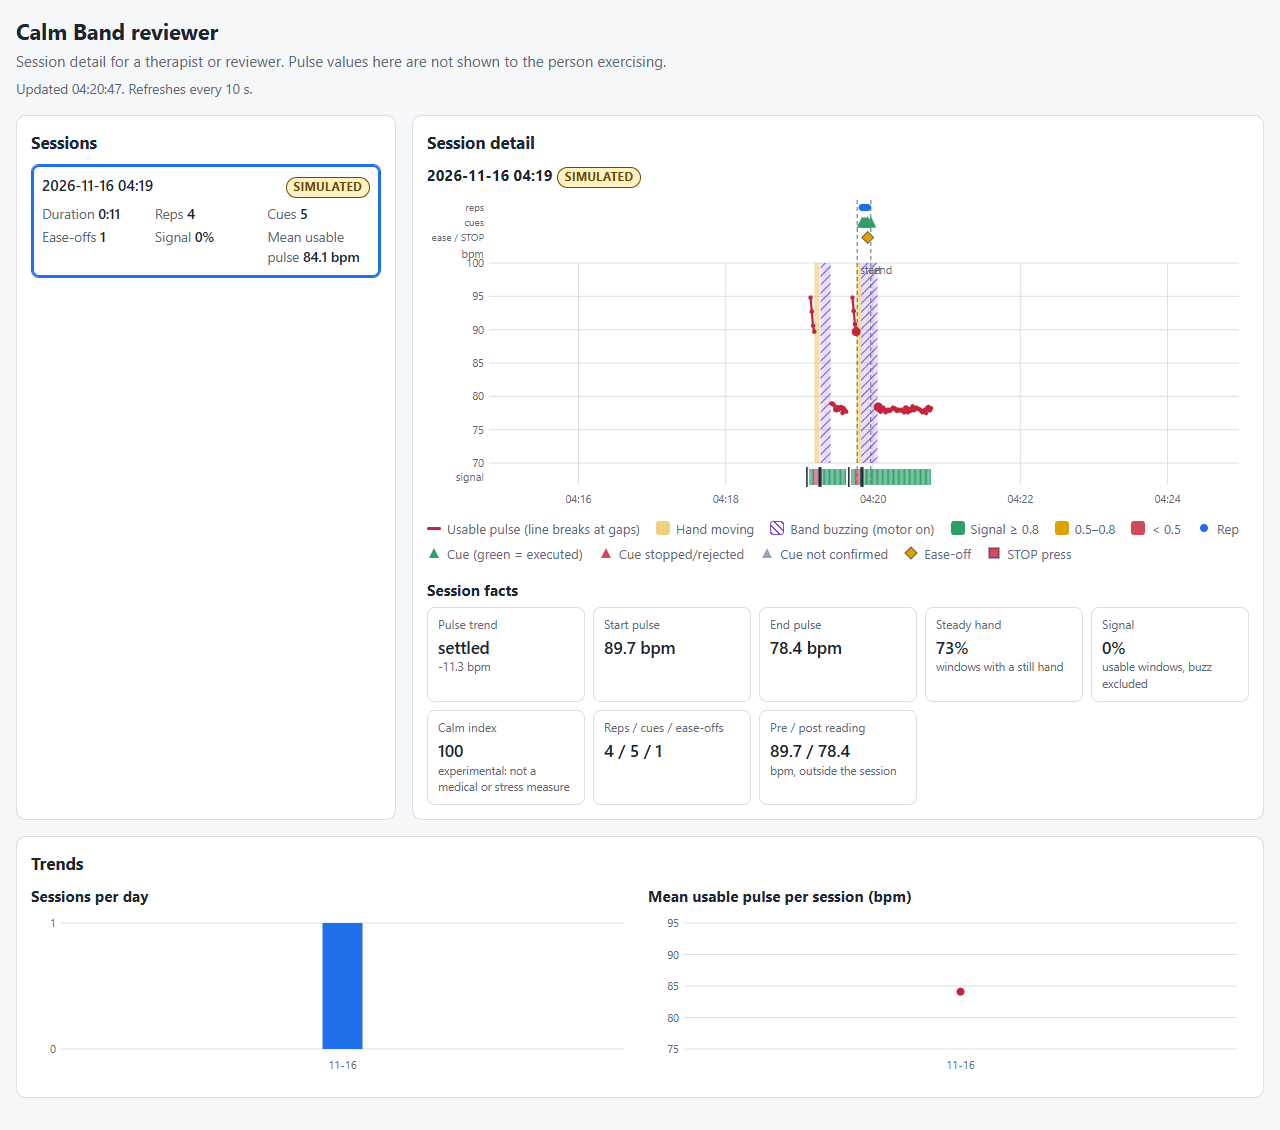
\includegraphics[width=6.0in,height=4.4in,keepaspectratio]{integrated-reviewer-list.png}\caption{Reviewer Page: Session List, Session Facts and Trends}\label{fig:rev_list}\end{figure}

\begin{figure}[H]\centering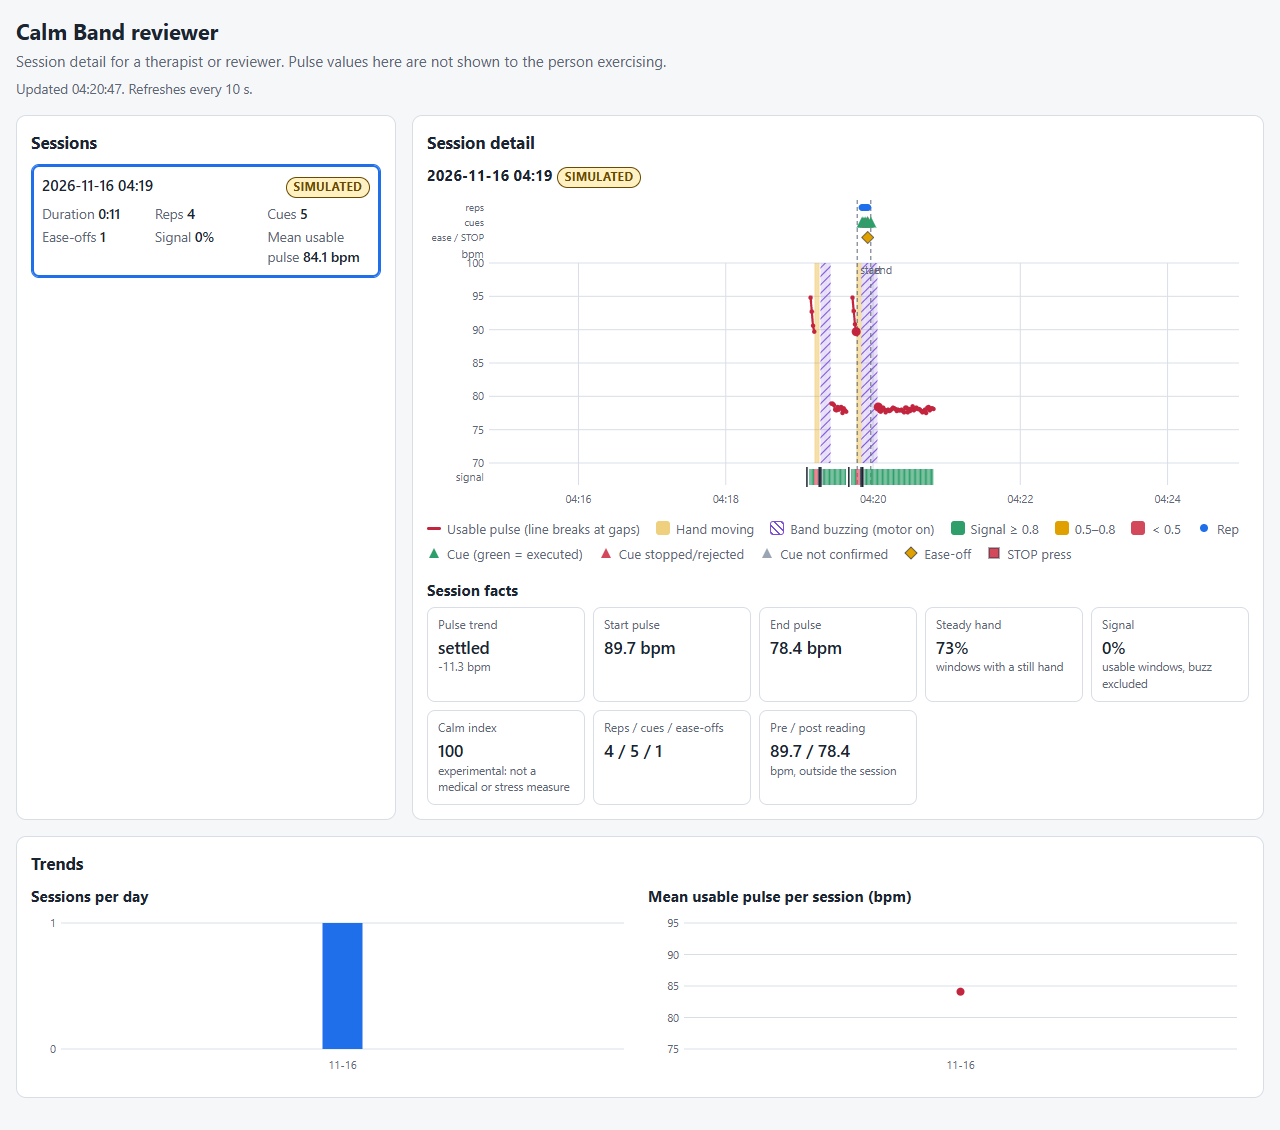
\includegraphics[width=6.0in,height=4.4in,keepaspectratio]{integrated-reviewer-timeline.png}\caption{Reviewer Page: Session Timeline with Gaps, Buzz and Movement Shading and Markers}\label{fig:rev_timeline}\end{figure}

\section{Experimental Calm Index}\label{sec:6.calm}

The reviewer page also shows one derived number, the \textbf{calm index}. It compares the pulse at the end of a session with the pulse at its start. Only \emph{clean} windows are used (no buzz, no movement, quality at least 0.8, contact present, no timing gap); the last clean window before the session and the first clean window after it are included, because the windows inside a session are mostly disturbed by cues. With $s$ the first and $e$ the last clean pulse of the session in beats per minute, the index is
\begin{equation*}
\text{calm index} = \operatorname{round}\Bigl(100 \times \operatorname{clamp}\bigl(\tfrac{s - e}{15} + 0.5,\ 0,\ 1\bigr)\Bigr).
\end{equation*}
A value of 50 means the same pulse as at the start; 100 means a drop of 7.5 BPM or more; 0 means a rise of 7.5 BPM or more. With fewer than two clean readings the value is missing, not zero. The index is always printed with the label \textbf{``experimental: not a medical or stress measure''}. It compares a person only with their own start of that one session, so it cannot be compared between people or sessions. MirrorWell does not show it at all.

\section{Experimental Stress Model (WESAD)}\label{sec:6.stress}

A small stress model was trained and tested offline on the public WESAD dataset [8] (Schmidt et al., ICMI 2018). It uses the wrist pulse signal (blood-volume pulse) recorded by the Empatica E4 at 64 Hz from 15 subjects (S2 to S17, without S12), and only the \emph{baseline} (sitting calmly) and \emph{stress} (a public-speaking and mental-arithmetic task) segments. Windows of 60 seconds were taken every 15 seconds, and windows with fewer than 20 valid beat intervals were dropped. This leaves \textbf{1,592 windows}, 33\% of them from the stress task. WESAD is for non-commercial scientific use, so the data is not stored in the project.

The model sees three numbers per window: the average pulse, the beat-to-beat variation of the pulse, and how far the pulse is above that person's own calm baseline. Every model was tested with \textbf{leave-one-subject-out} evaluation: it is trained on 14 people, tested on the 15th, and this is repeated for each person. Table~\ref{tab:stress-model-results} gives the mean and standard deviation over the 15 people. Balanced accuracy counts calm and stress equally, so 0.5 is a coin flip.

\begin{table}[H]
\centering\small\setstretch{1.0}
\caption{Leave-One-Subject-Out Results of the Experimental Stress Model on WESAD}\label{tab:stress-model-results}
\begin{tabular}{|>{\raggedright\arraybackslash}p{\dimexpr 0.30\linewidth-2\tabcolsep-0.4pt\relax}|>{\raggedright\arraybackslash}p{\dimexpr 0.28\linewidth-2\tabcolsep-0.4pt\relax}|>{\raggedright\arraybackslash}p{\dimexpr 0.21\linewidth-2\tabcolsep-0.4pt\relax}|>{\raggedright\arraybackslash}p{\dimexpr 0.21\linewidth-2\tabcolsep-0.4pt\relax}|}
\hline
\rowcolor{headgray}\textbf{Model} & \textbf{Features} & \textbf{Balanced accuracy} & \textbf{F1 (stress)} \\ \hline
Majority class & none & 0.500 ± 0.000 & 0.000 ± 0.000 \\ \hline
Threshold rule & relative pulse & 0.813 ± 0.144 & 0.716 ± 0.236 \\ \hline
Logistic regression v1 & all 3 & 0.803 ± 0.133 & 0.702 ± 0.217 \\ \hline
Logistic regression v1b & pulse + relative pulse & 0.802 ± 0.160 & 0.707 ± 0.246 \\ \hline
Random forest (comparison) & all 3 & 0.804 ± 0.130 & 0.710 ± 0.212 \\ \hline
\end{tabular}
\end{table}

All three real models reach about 0.80. A one-line threshold on the relative pulse is as good as logistic regression or a random forest, so the model is not doing anything complicated; the personal baseline carries most of the signal. The results also vary a lot between people (standard deviation 0.13 to 0.16): for some people it works well, for others it is close to guessing.

\textbf{Why v1b drops pulse variability.} Version v1b keeps the same layout as v1 but switches off the beat-to-beat variation feature. This costs nothing measurable on WESAD (0.802 against 0.803), although it is a little less consistent between people. The reason is a \textbf{sensor mismatch}: the variation in the WESAD windows averages about 16 BPM, while our MAX30102 band reads roughly 2 to 7 BPM, so that feature would fall far outside the range the model was trained on.

\textbf{Status.} The model is shown only on the reviewer page and is labelled \textbf{experimental}; MirrorWell does not show it. It is \textbf{not validated on our band}: the Empatica E4 has a different signal quality, placement and sampling rate, and the test compared a laboratory stress task with sitting still, so exercise, caffeine, excitement or talking can also raise the score. It also needs a calm baseline from the same person, and it was tested on 15 mostly young volunteers. It is a biofeedback aid, not a medical or diagnostic tool.

\section{Testing of the New Parts}\label{sec:6.newtests}

The new parts were tested automatically at several levels (Table~\ref{tab:new-tests}) and then end to end. The counts below are from the final merged build.

\begin{table}[H]
\centering\small\setstretch{1.0}
\caption{Automated Tests of the Storage, Live Card, Summary and Reviewer Parts}\label{tab:new-tests}
\begin{tabular}{|>{\raggedright\arraybackslash}p{\dimexpr 0.28\linewidth-2\tabcolsep-0.4pt\relax}|>{\raggedright\arraybackslash}p{\dimexpr 0.56\linewidth-2\tabcolsep-0.4pt\relax}|>{\raggedright\arraybackslash}p{\dimexpr 0.16\linewidth-2\tabcolsep-0.4pt\relax}|}
\hline
\rowcolor{headgray}\textbf{Suite} & \textbf{What it covers} & \textbf{Result} \\ \hline
Backend UI checks & Storage and restart, live, summary, reviewer and trend endpoints, calm index, origin labels & 181 / 181 \\ \hline
Backend status checks & The original status rules, unchanged by the database & 33 / 33 \\ \hline
MirrorWell tests & Whole MirrorWell test suite, including the live card and summary & 438 / 438 \\ \hline
Reviewer page tests & Reviewer page against the example data: list, timeline, trends, empty and error cases, phone and dark layouts & Pass \\ \hline
\end{tabular}
\end{table}

The \textbf{integrated run} started the real backend, the real MirrorWell pages and the reviewer page together with the \emph{simulated} band, played a short session and produced the screenshots in Figures~\ref{fig:ui_live_cue}, \ref{fig:ui_summary}, \ref{fig:rev_list} and~\ref{fig:rev_timeline}. All of this testing used the simulated band, whose pulse is synthetic and is labelled as such. \textbf{A real-band session with these new screens is checked at the demonstration}; it was not done before this report was written.

\section{Discussion}\label{sec:6.4}

The results support the design's central idea: that a low-cost IoT companion can be both useful and honest about its data. The strict flags and status rules mean that the user sees a pulse value only when it can be trusted, and the reviewer sees exactly why other readings were withheld. The command rules ensure that a delayed, duplicated or malformed message cannot cause an unexpected vibration, and the local STOP button means the user is always in control.


The review process proved valuable. Each round found real defects that the existing tests did not cover, several of which only appear under timing or failure conditions (a blocked network loop, a sensor failing mid-session, a brief finger removal between two windows). Writing a failing test for each finding before fixing it prevented regressions in later rounds.


The vibration-overlap policy has a cost: frequent rep cues leave few clean windows inside a session, so Phase 1 relies on before and after readings. This is a deliberate trade-off in favour of trustworthy data until real measurements show how long a cue actually disturbs the signal.


\section{Limitations}\label{sec:6.5}

\begin{itemize}\item The physical prototype was tested by the team on one person over two days (Section~\ref{sec:6.hw}). The resting pulse has not been checked against a manual count or a reference device, and how long a buzz disturbs the pulse signal has not yet been measured.
\item The contact check (raw IR ≥ 50,000) can be passed by a reflective surface: with the sensor face-down on a table it reported a false pulse. Correct handling (sensor face-up, finger resting lightly) avoids this for now.
\item The encrypted EMQX connection is implemented in the firmware but has not been tested end to end; the simulator, the test backend and the hardware test all used a local broker without TLS.
\item The backend stores data in a local SQLite file on one laptop; a cloud database is not connected. The new live card, summary and reviewer page were tested with the simulated band; their check with the real band is done at the demonstration. The calm index is experimental and is not a medical or stress measure.
\item The experimental stress model was trained and tested only on WESAD (Empatica E4); it has not been validated on our band.
\end{itemize}

\chapter{CONCLUSION AND FUTURE SCOPE}\label{ch:7}

\section{Conclusion}\label{sec:7.1}

This project designed and implemented the Calm Band, an IoT companion that adds pulse and motion sensing and safe haptic cues to MirrorWell's facial-exercise sessions. The system follows a classic IoT architecture (wearable sensors, an ESP32 hub, an MQTT broker and a FastAPI backend) within a hardware budget of ₹949–1,449. Its distinguishing feature is that data quality and actuation safety are built into every layer: readings carry explicit contact, motion, vibration and timing flags; the backend withholds any reading it cannot trust; and vibration commands are validated, time-limited and locally stoppable.


The firmware compiles for the ESP32 using 69\% of flash and 35\% of RAM, all 117 automated checks pass, and emulator self-tests confirm that sensing and vibration timing are independent of network delays. The physical prototype confirmed these results on real parts: it produced a usable resting pulse with quality up to 1.00, executed every vibration cue from a live MirrorWell session, withheld the pulse when the finger was removed or the band moved, and recovered from an 85-second network loss without losing any data.


The demonstration build adds the parts a user and a therapist actually see. MirrorWell now shows a live band card with a heart that beats at the measured pace, signal bars, steadiness and a settling arrow, with no raw numbers and with honest messages when the data is poor, and it ends each session with a summary in plain words. A reviewer page shows each session as a timeline with gaps left empty, marks buzzes, movement, cues and STOP presses, labels simulated data, and offers an experimental calm index. Session data now survives backend restarts in SQLite, and an experimental WESAD-trained stress model (balanced accuracy about 0.80 in leave-one-subject-out tests, not yet validated on the band) is shown on the reviewer page only. These parts passed 181 backend UI checks, the 33 backend checks, 438 MirrorWell tests and the reviewer page tests with the simulated band; the real-band session with these screens is checked at the demonstration.


\section{Future Scope}\label{sec:7.2}

\begin{enumerate}\item \textbf{Hardware validation:} compare the band's pulse with a manual count or a reference pulse oximeter, add a plausibility check (for example, rejecting windows with a very high beat-to-beat spread) so that a reflective surface cannot pass as a finger, and measure the motor's interference on the pulse sensor.
\item \textbf{Validate the stress model on the band:} the WESAD-trained model (logistic regression and random forest, leave-one-subject-out) has not been tested on our band's signal; record sessions with the band, compare the model with them, and find a variability feature that suits the MAX30102.
\item \textbf{RMSSD in the firmware:} compute this beat-to-beat variability measure on the band itself from the clean beat intervals.
\item \textbf{Data collection and personal calibration:} record a small dataset in RECORD mode and calibrate the model to each person.
\item \textbf{Live model scoring:} score the model on live windows during a session, with the same quality rules that apply today.
\item \textbf{Wearable enclosure and battery:} replace the breadboards with a compact, battery-powered enclosure worn on the wrist.
\item \textbf{Cloud broker and database:} test the full chain over a cloud MQTT broker with TLS and per-device credentials, give each band a unique MQTT client id, and move storage to a cloud database.
\item \textbf{Smart reminders:} add session reminders and adherence tracking, and serve the companion over HTTPS for phones.
\item \textbf{Alternative sensing:} an open-protocol smart ring (such as the Colmi R02) could replace the wired fingertip and wrist sensors while the ESP32 keeps the haptic role, reducing wiring.
\end{enumerate}

\clearpage
{\noindent\bfseries\fontsize{16}{22}\selectfont REFERENCES}\label{refs}\par\vspace{8pt}
{\setstretch{1.1}\setlength{\parskip}{6pt}
\noindent[1] L. Atzori, A. Iera and G. Morabito, "The Internet of Things: A survey," Computer Networks, vol. 54, no. 15, pp. 2787–2805, 2010.\par
\noindent[2] S. M. R. Islam, D. Kwak, M. H. Kabir, M. Hossain and K.-S. Kwak, "The Internet of Things for Health Care: A Comprehensive Survey," IEEE Access, vol. 3, pp. 678–708, 2015.\par
\noindent[3] J. Allen, "Photoplethysmography and its application in clinical physiological measurement," Physiological Measurement, vol. 28, no. 3, pp. R1–R39, 2007.\par
\noindent[4] T. Tamura, Y. Maeda, M. Sekine and M. Yoshida, "Wearable Photoplethysmographic Sensors—Past and Present," Electronics, vol. 3, no. 2, pp. 282–302, 2014.\par
\noindent[5] C. Lugaresi et al., "MediaPipe: A Framework for Building Perception Pipelines," arXiv:1906.08172, 2019.\par
\noindent[6] L. M. Pereira, K. Obara, J. M. Dias, M. O. Menacho, E. L. Lavado and J. R. Cardoso, "Facial exercise therapy for facial palsy: systematic review and meta-analysis," Clinical Rehabilitation, vol. 25, no. 7, pp. 649–658, 2011.\par
\noindent[7] H.-G. Kim, E.-J. Cheon, D.-S. Bai, Y. H. Lee and B.-H. Koo, "Stress and Heart Rate Variability: A Meta-Analysis and Review of the Literature," Psychiatry Investigation, vol. 15, no. 3, pp. 235–245, 2018.\par
\noindent[8] P. Schmidt, A. Reiss, R. Duerichen, C. Marberger and K. Van Laerhoven, "Introducing WESAD, a Multimodal Dataset for Wearable Stress and Affect Detection," in Proc. 20th ACM International Conference on Multimodal Interaction (ICMI), 2018, pp. 400–408.\par
\noindent[9] OASIS, "MQTT Version 3.1.1," OASIS Standard, A. Banks and R. Gupta, Eds., 2014.\par
\noindent[10] M. Elgendi, "On the Analysis of Fingertip Photoplethysmogram Signals," Current Cardiology Reviews, vol. 8, no. 1, pp. 14–25, 2012.\par
\noindent[11] Maxim Integrated, "MAX30102: High-Sensitivity Pulse Oximeter and Heart-Rate Sensor for Wearable Health," datasheet, Rev. 1, 2018.\par
\noindent[12] Y. S. Can, B. Arnrich and C. Ersoy, "Stress detection in daily life scenarios using smart phones and wearable sensors: A survey," Journal of Biomedical Informatics, vol. 92, 103139, 2019.\par
\noindent[13] InvenSense, "MPU-6000 and MPU-6050 Product Specification," Rev. 3.4, 2013.\par
\noindent[14] M. S. Schwartz and F. Andrasik, Eds., Biofeedback: A Practitioner's Guide, 4th ed. New York: Guilford Press, 2016.\par
\noindent[15] Espressif Systems, "ESP32 Series Datasheet," Version 4.x, Espressif Systems, Shanghai.\par
}

\clearpage\fronttitle{APPENDICES}\label{appx}
\setcounter{table}{0}\renewcommand{\thetable}{A.\arabic{table}}

\section*{Appendix 1: Message Formats}\label{sec:appendix-1-message-formats}

\textbf{Feature window} (published every 15 seconds on \texttt{calmband/\allowbreak{}cb-01/\allowbreak{}features}):


\begin{lstlisting}
{"schema":1,"dev":"cb-01","boot":"91ce996b","seq":17,"origin":"live",
 "windowStartMs":1760000030003,"windowEndMs":1760000090003,"clockValid":true,
 "contact":true,"quality":1.00,"pulseRateBpm":76.4,"pulseRateSdBpm":0.49,
 "validBeatFraction":1.00,"validIbis":72,"motionValid":true,"motionCoverage":1.00,
 "motionRms_g":0.0120,"motionMax_g":0.031,"moving":false,
 "motorActive":false,"timingGap":false}
\end{lstlisting}

\textbf{Status} (retained on \texttt{calmband/\allowbreak{}cb-01/\allowbreak{}status}):


\begin{lstlisting}
{"dev":"cb-01","boot":"91ce996b","online":true,"clockValid":true,
 "droppedWindows":0,"publishFailures":0,"pulseSensor":"ok","motionSensor":"ok"}
\end{lstlisting}

\textbf{Command} (backend to band on \texttt{calmband/\allowbreak{}cb-01/\allowbreak{}cmd}) and \textbf{acknowledgement}:


\begin{lstlisting}
{"commandId":"6f1c2a9e","sessionId":"cs-1a2b3c4d","pattern":"rep_pulse",
 "maxDurationMs":1500,"issuedAtMs":1760000040000,"expiresAtMs":1760000043000}

{"commandId":"6f1c2a9e","dev":"cb-01","boot":"91ce996b",
 "result":"executed","reason":null,"atMs":1760000040300}
\end{lstlisting}

\section*{Appendix 2: Bill of Materials}\label{sec:appendix-2-bill-of-materials}

\begin{table}[H]
\centering\small\setstretch{1.0}
\caption{Bill of Materials (estimated prices, October 2026)}\label{tab:bill-of-materials-estimated-prices-octob}
\begin{tabular}{|>{\raggedright\arraybackslash}p{\dimexpr 0.582\linewidth-2\tabcolsep-0.4pt\relax}|>{\raggedright\arraybackslash}p{\dimexpr 0.145\linewidth-2\tabcolsep-0.4pt\relax}|>{\raggedright\arraybackslash}p{\dimexpr 0.242\linewidth-2\tabcolsep-0.4pt\relax}|}
\hline
\rowcolor{headgray}\textbf{Item} & \textbf{Qty} & \textbf{Estimated cost (₹)} \\ \hline
ESP32 DevKit V1 (ESP32-WROOM-32, 30-pin) & 1 & 400–550 \\ \hline
MAX30102 pulse sensor module & 1 & 150–250 \\ \hline
MPU6050 (GY-521) motion sensor & 1 & 100–150 \\ \hline
Vibration motor module (driver + diode) & 1 & 59 \\ \hline
Tactile push button 6 × 6 mm & 2 & 10–20 \\ \hline
Male-to-female jumpers, 30 cm (strip) & 20–40 & 60–100 \\ \hline
Male-to-male jumpers, 10 cm & a few & 20–40 \\ \hline
Mini breadboard, 170 holes & 2 & 50–80 \\ \hline
Velcro, 2–2.5 cm wide & about 1 m & 50–100 \\ \hline
Delivery & 1 order & 50–100 \\ \hline
\rowcolor{totalgray}\textbf{Total (must-buy items)} & \textbf{} & \textbf{949–1,449} \\ \hline
\end{tabular}
\end{table}

Household mounting items (foam, tape, cable ties) add ₹110–260 if not already available; header pins, solder and capacitors (₹70–140) are usually available in the lab.


\section*{Paper Publication Proof}\label{sec:paper-publication-proof}

[To be attached.]


\section*{Plagiarism Report}\label{sec:plagiarism-report}

[To be attached.]

\end{document}
